\documentclass{article}
\usepackage[utf8]{inputenc}
\usepackage[multiple]{footmisc}
\usepackage[a4paper, total={6in, 8in}]{geometry}

%\usepackage{graphicx}
%\graphicspath{ {./images/} }

\usepackage{svg}
\usepackage{float}
\usepackage{amsmath} 
\usepackage{tabulary} 

\title{LUSC-A-12 LSST:UK phase A alert handling infrastructure experiments}
\author{D. Morris}
\date{June 2020}

\setlength{\parskip}{1em}

%\usepackage{natbib}
%\bibliographystyle{abbrvnat}
%\setcitestyle{authoryear,open={((},close={))}}

% burl doesn't work in pdflatex
% https://tex.stackexchange.com/a/212921
%\usepackage{breakurl}

\usepackage[style=numeric]{biblatex}
\addbibresource{references.bib}

\usepackage{xspace}
% Standard terms used throughout the document,
% defined as macro commands to maintain consistency
\newcommand{\json} {JSON\xspace}
\newcommand{\yaml} {YAML\xspace}
\newcommand{\avro} {Avro\xspace}
\newcommand{\fits} {FITS\xspace}
\newcommand{\png} {PNG\xspace}
\newcommand{\jpeg} {JPEG\xspace}
\newcommand{\parquet} {Parquet\xspace}
\newcommand{\votable} {VOTable\xspace}
\newcommand{\voevent} {VOEvent\xspace}

\newcommand{\ansible} {Ansible\xspace}
\newcommand{\docker} {Docker\xspace}
\newcommand{\dockercompose} {docker-compose\xspace}
\newcommand{\terraform} {Terraform\xspace}
\newcommand{\kubernetes} {Kubernetes\xspace}

\newcommand{\openstack} {Openstack\xspace}
\newcommand{\dnsmasq} {\texttt{dnsmasq}\xspace}
\newcommand{\dns} {DNS\xspace}
\newcommand{\dhcp} {DCHP\xspace}
\newcommand{\ceph} {Ceph\xspace}
\newcommand{\cephfs} {CephFS\xspace}

\newcommand{\ischnura} {Ischnura\xspace}
\newcommand{\esperia} {Esperia\xspace}
\newcommand{\enteucha} {Enteucha\xspace}

\newcommand{\libvirt} {\texttt{libvirt}\xspace}
\newcommand{\cloudinit} {\texttt{cloud-init}\xspace}
\newcommand{\kickstart} {kickstart\xspace}
\newcommand{\sysadmin} {system-admin\xspace}
\newcommand{\stevedore} {\textit{Stevedore}\xspace}

\newcommand{\btrfs} {\texttt{btrfs}\xspace}
\newcommand{\filesystem} {file-system\xspace}
\newcommand{\scaleable} {scaleable\xspace}

\newcommand{\centre} {centre\xspace}
\newcommand{\centred} {centred\xspace}

\newcommand{\paas} {PaaS\xspace}
\newcommand{\datacentre} {datacentre\xspace}
\newcommand{\datacentres} {datacentres\xspace}
\newcommand{\webservice} {webservice\xspace}
\newcommand{\webservices} {webservices\xspace}

\newcommand{\redhat} {RedHat\xspace}
\newcommand{\fedora} {Fedora\xspace}

\newcommand{\github} {GitHub\xspace}

\newcommand{\kafka} {Kafka\xspace}
\newcommand{\flink} {Flink\xspace}
\newcommand{\spark} {Spark\xspace}
\newcommand{\cassandra} {Cassandra\xspace}
\newcommand{\zookeeper} {Zookeeper\xspace}

\newcommand{\kftopic} {\textit{topic}\xspace}
\newcommand{\kftopics} {\textit{topics}\xspace}
\newcommand{\kfstream} {\textit{stream}\xspace}
\newcommand{\kfstreams} {\textit{streams}\xspace}
\newcommand{\kfbroker} {\textit{broker}\xspace}
\newcommand{\kfbrokers} {\textit{brokers}\xspace}
\newcommand{\kfconsumer} {\textit{consumer}\xspace}
\newcommand{\kfconsumers} {\textit{consumers}\xspace}
\newcommand{\kfproducer} {\textit{producer}\xspace}
\newcommand{\kfproducers} {\textit{producers}\xspace}
\newcommand{\kfpublisher} {\textit{publisher}\xspace}
\newcommand{\kfpublishers} {\textit{publishers}\xspace}
\newcommand{\kfsubscriber} {\textit{subscriber}\xspace}
\newcommand{\kfsubscribers} {\textit{subscribers}\xspace}

\newcommand{\kfpartition} {\textit{partition}\xspace}
\newcommand{\kfpartitions} {\textit{partitions}\xspace}

\newcommand{\apache} {Apache\xspace}
\newcommand{\confluent} {Confluent\xspace}

\newcommand{\virtualbox} {VirtualBox\xspace}
\newcommand{\vagrant} {Vagrant\xspace}
\newcommand{\kvm} {KVM\xspace}
\newcommand{\vlan} {VLAN\xspace}

\newcommand{\fifo} {FIFO\xspace}
\newcommand{\junit} {JUnit\xspace}

\newcommand{\mariadb} {MariaDB\xspace}
\newcommand{\hsqldb} {HSQLDB\xspace}
\newcommand{\cqengine} {CQEngine\xspace}
\newcommand{\htmid} {HTMID\xspace}
\newcommand{\crossmatch} {crossmatch\xspace}
\newcommand{\crossmatcher} {crossmatcher\xspace}
\newcommand{\crossmatching} {crossmatching\xspace}
\newcommand{\benchmark} {benchmark\xspace}
\newcommand{\benchmarking} {benchmarking\xspace}
\newcommand{\dataset} {dataset\xspace}

\newcommand{\catalog} {catalog\xspace}
\newcommand{\catalogs} {catalogs\xspace}

\newcommand{\avschema} {\textit{schema}\xspace}
\newcommand{\avschemas} {\textit{schema}\xspace}
\newcommand{\conschemareg} {registry\xspace}
\newcommand{\conschemaregs} {registries\xspace}
\newcommand{\conschemaregistry} {Schema Registry\xspace}
\newcommand{\mirrormaker} {Mirror Maker\xspace}

\newcommand{\serz}      {serialize\xspace}
\newcommand{\serzed}    {serialized\xspace}
\newcommand{\serzer}    {serializer\xspace}
\newcommand{\serzers}   {serializers\xspace}
\newcommand{\deserz}    {deserialize\xspace}
\newcommand{\deserzed}  {deserialized\xspace}
\newcommand{\deserzer}  {deserializer\xspace}
\newcommand{\deserzers} {deserializers\xspace}
\newcommand{\deserzing} {deserializing\xspace}

\newcommand{\phasea} {phase A\xspace}
\newcommand{\phaseb} {phase B\xspace}
\newcommand{\stageone} {stage 1\xspace}
\newcommand{\stagetwo} {stage 2\xspace}
\newcommand{\stagethr} {stage 3\xspace}

\newcommand{\ztf} {ZTF\xspace}
\newcommand{\lsst} {LSST\xspace}
\newcommand{\lsstuk} {LSST:UK\xspace}
\newcommand{\lasair} {Lasair\xspace}

\newcommand{\gaia} {Gaia\xspace}
\newcommand{\cunine} {CU9\xspace}

\newcommand{\cam} {Cambridge\xspace}
\newcommand{\ral} {RAL\xspace}
\newcommand{\roe} {ROE\xspace}
\newcommand{\wfau} {WFAU\xspace}
\newcommand{\iris} {IRIS\xspace}
\newcommand{\uedin} {University of Edinburgh\xspace}
\newcommand{\testplatform} {test platform\xspace}

\newcommand{\eleanor} {Eleanor\xspace}
\newcommand{\cumulus} {Cumulus\xspace}

\newcommand{\hdisk} {disk\xspace}

\newcommand{\footurl}[1] {\footnote{\url{#1}}}

\usepackage{color}
\usepackage{listings}
\usepackage{changepage}

\usepackage{courier}
%\usepackage{beramono}


\lstset{basicstyle=\ttfamily\small}
\lstset{basewidth={0.5em,0.5em}}

\definecolor{codeblue}{RGB}{42,0,255}
\definecolor{codegreen}{RGB}{63,127,95}
\definecolor{codelilac}{RGB}{127,0,85}

\lstloadlanguages{Java}
\lstdefinestyle{Java}{
    language=Java,
    identifierstyle=\color{codeblue},
    commentstyle=\color{codegreen}\textit,
    keywordstyle=\color{codelilac},
    keepspaces=true,
    morekeywords={enum},
    }

\newcommand{\javaname}[1] {{\ttfamily\color{codeblue} #1}}
\newcommand{\javaplural}[1] {\javaname{#1}s}

\lstloadlanguages{SQL}
\lstdefinestyle{SQL}{
    language=SQL,
    commentstyle=\color{codegreen}\textit,
    keepspaces=true,
    keywordstyle=\color{codeblue},
    morekeywords={enum},
    }

% YAML formatting.
% https://tex.stackexchange.com/questions/152829/how-can-i-highlight-yaml-code-in-a-pretty-way-with-listings

% \usepackage[dvipsnames]{xcolor}
\newcommand\YAMLcolonstyle{\ttfamily\small\color{codeblue}}
\newcommand\YAMLkeystyle{\ttfamily\small\color{codeblue}}
\newcommand\YAMLvaluestyle{\ttfamily\small\color{codegreen}}

\makeatletter
% here is a macro expanding to the name of the language
% (handy if you decide to change it further down the road)
\newcommand\language@yaml{yaml}

\expandafter\expandafter\expandafter\lstdefinelanguage
\expandafter{\language@yaml}{
    keywords={true,false,null,y,n},
    keywordstyle=\color{codeblue},
    basicstyle=\YAMLkeystyle, % assuming a key comes first
    sensitive=false,
    comment=[l]{\#},
    morecomment=[s]{/*}{*/},
    commentstyle=\color{codegreen}\textit,
    stringstyle=\color{codegreen}\textit,
    moredelim=[l][\color{orange}]{\&},
    moredelim=[l][\color{magenta}]{*},
    moredelim=**[il][\YAMLcolonstyle{:}\YAMLvaluestyle]{:}, % switch to value style at :
    morestring=[b]',
    morestring=[b]",
    literate =  {---}{{\ProcessThreeDashes}}3
                {>}{{\textcolor{red}\textgreater}}1     
                {|}{{\textcolor{red}\textbar}}1 
                {\ -\ }{{\mdseries\ -\ }}3,
}

% switch to key style at EOL
\lst@AddToHook{EveryLine}{\ifx\lst@language\language@yaml\YAMLkeystyle\fi}
\makeatother
\newcommand\ProcessThreeDashes{\llap{\color{codegreen}\mdseries-{-}-}}

\begin{document}

\maketitle

%Push text to the bottom of the page.
%https://tex.stackexchange.com/a/300368
\vspace*{\fill}
This work has been supported by STFC funding for UK participation in LSST, through grant ST/N002512/1.

%TODO Citeable DOI GitHub repositories.
%https://academia.stackexchange.com/a/20999
%https://github.blog/2014-05-14-improving-github-for-science/
%https://guides.github.com/activities/citable-code/
\clearpage

\tableofcontents
\clearpage

\section{Introduction}
\label{introduction}
This document describes some experiments designed to address some of the challenges we expect to encounter implementing a scalable architecture for a real-time alert processing system for the \lsstuk\footurl{https://www.lsst.ac.uk/} project capable of handling the data rates expected during the lifetime of the \lsst\footurl{https://www.lsst.org/} project.

The design criteria for the system include the following requirements:
\begin{itemize}
  \item Capable of meeting the initial expected data rate from the \lsst project.
  \item The ability to increase the processing speed of the system by adding new resources.
  \item The ability to increase the storage capacity of the system by adding new resources.
  \item Minimising the downtime required to add new resources to the system.
  \item The resilience of the system to individual component failures.
\end{itemize}

Additional criteria set by the requirements of the \lsstuk project and the planned deployment on resources provided by the \iris eInfrastructure initiative\footurl{https://www.iris.ac.uk/}:
\begin{itemize}
  \item It should be possible to implement the system using standard hardware resources.
  \item It should be possible to deploy the system on generic cloud compute resources.
\end{itemize}

The target data rates for the experiments are:
\begin{itemize}
  \item Sustained 1,000 alerts per second.
  \item Stretch goal 10,000 alerts per second.
\end{itemize}

These numbers are based on the values given in table 29 of the \lsst System Science Requirements Document (LPM-17)\footurl{https://docushare.lsst.org/docushare/dsweb/Get/LPM-17}.

\begin{quote}
\textit{“Specification: The system should be capable of reporting such data for at least transN candidate transients per field of view and visit”}
\end{quote}

\begin{center}
\begin{tabular}{|l|l|l|l|}
\hline
\textit{Quantity} & \textit{DesignSpec} & \textit{MinimumSpec} & \textit{StretchGoal} \\ \hline
\textit{transN}   & $10^{4}$            & $10^{3}$             & $10^{5}$             \\ \hline
\end{tabular}
\end{center}

The \textit{transN} value sets the number of alerts per visit, this combined with the expected cadence of 30 seconds per visit gives us our target evaluation criteria of 1,000 alerts per second and the stretch goal of 10,000 alerts per second for these experiments.

To meet the scalability and fault tolerance requirements we developed a micro-service\footurl{https://microservices.io/} based design for the alert processing system, where multiple instances of each component can be deployed in parallel, using \kafka\footurl{https://kafka.apache.org/} to distribute the alerts between components in the pipeline.

Our initial reason for selecting \kafka as the message transport technology was informed by the work done by M. Patterson\cite{Patterson-2018} and colleagues developing the alert processing infrastructure for the Zwicky Transient Facility (ZTF)\footurl{https://www.ztf.caltech.edu/} project.

The \ztf alert processing infrastructure is considered a prototype for the \lsst alert processing infrastructure, which is planning to use a similar \kafka based system as the primary distribution protocol for the \lsst level 1 alert stream.

Both of these are examples of using \kafka as an external site to site delivery protocol.
However, \kafka was originally designed as an internal message delivery system for data streams processing applications within a \datacentre, rather than an external site to site delivery system.
As we learned more about \kafka and its capabilities it became clear that it would be an ideal technology for implementing the internal data streams linking together individual micro-service components within our system, enabling us to build a flexible and \scaleable system.

\section{High level outline}
\label{high-level-outline}

The proposed architecture design consists of three layers of components, connected together by \kafka streams.

\subsection{Stage 1, input buffer}
\label{stage-1}

The first stage of the system architecture is a local \kafka mirror configured as a 7 day first-in first-out (\fifo) buffer of the live stream from \lsst. This buffer has a number of functions.

\subsubsection{Local endpoint}
\label{stage-1.local-endpoint}
Access to the upstream \kafka endpoint provided by \lsst is bandwidth limited, and will be limited to a small group of clients who are allowed to connect. Even if these restrictions are relaxed it will still make sense for each project to only make one connection to the upstream service.
This is particularly relevant in our case, as our connection to the upstream service involves a trans-Atlantic connection.
Implementing a mirror of the upstream service will provide a local \kafka endpoint for the rest of our components to connect to, enabling multiple components to connect to the primary input \kafka stream without placing an unnecessary load on our external network connection or the upstream service.

\subsubsection{Local buffer}
\label{stage-1.local-buffer}
Configuring our mirror of the upstream service as a 7 day \fifo buffer, makes our system more resilient to networking issues and component failures.
If a component in our system fails, the buffer gives us time to fix the issue, test and restart the failed component using data from our local buffer.

\subsubsection{Partition count}
\label{stage-1.partition-count}
The number of \kfpartitions in a \kafka stream puts an upper limit on the level of parallelism that downstream components can apply to processing a stream (see section \ref{kafka-partitions}).
Deploying a buffer at the input to our system give us direct control over the number of \kfpartitions available to the rest of our processing components.

\subsubsection{Schema mapping}
\label{stage-1.schema-mapping}
The ZTF and LSST alert messages are encoded using the \apache\avro\footurl{https://avro.apache.org/} binary encoding format. 

In addition to the binary message content, the live stream from \ztf includes an inline \avschema to describe the messages. Every message carries a copy of its \avschema; embedded in the message header \serzed as a plain text \json\footurl{https://www.json.org/} document.
This means the alert messages are self-describing, and provides some insulation from side effects of \avschema changes for clients.
However, embedding the \avschema in every message adds a non-trivial overhead, particularly if the stream only contains a small number of well known message types.

Our understanding is that the \lsst project intends to use a service similar to the \confluent \conschemaregistry\footurl{https://www.confluent.io/confluent-schema-registry/} to manage their \avro \avschema, and each message will only include a \avschema identifier rather than the full \avschema. This reduces the overhead associated with using an inline \avschema to describe the messages. However, the \avschema identifier will be specific to the upstream project's \conschemareg. This means we will need to provide a mapping from their \avschema identifiers to the corresponding \avschema identifiers in our own local \conschemareg.
This translation can be handled by the input buffer, replacing the upstream \avschema identifier with the corresponding local identifier as it receives the messages (see section \ref{avro-schema}).

\subsubsection{Topic merge}
\label{stage-1.topic-merge}
The current stream from \ztf is published as a series of separate daily \kftopics, one for each night of observations. Handling the data in chunks like this a useful format to manage the bulk transfer and archiving of the data. When making backups or managing data transfers it is convenient to be able to refer to [\textit{the data from yesterday}] or [\textit{the data from three days ago}]. However, our end users are more likely to want to access [\textit{the live data from \lsst}], in one continuous stream.

Ideally it would be useful to have access to both a single continuous \kfstream for the science use cases, and a series of separate daily \kftopics for system administration and backups.

Depending on how the live data stream from \lsst is configured, as a single continuous \kfstream or as separate daily \kfstreams, our \fifo buffer can either split the continuous \kfstream into separate \kftopics for the system administration tasks, or merge the separate \kftopics into one continuous \kfstream for our science uses.

By placing our own \fifo buffer at the head of our processing chain we are insulated from changes to the design of the upstream \kfstream from \lsst.
Our \fifo buffer would handle changes to the \kftopics and \avschema by the upstream service and present a consistent set of \kftopics and \avschema to our internal components.

\subsubsection{Test data}
\label{stage-1.test-data}
The same \kafka service can also provide access to a set of test data that will be useful for our own integration testing, and for end users developing and testing their own custom processors.

Example test data:
\begin{itemize}
  \item Known sets of simulated data for specific scenarios.
  \item Known subsets of historical data from \ztf.
  \item \ztf data with static, inline and registered \avschema.
  \item \lsst data with static, inline and registered \avschema.
\end{itemize}

The advantage of using the same \kafka service to store and serve test data is it means our components can use the same libraries and configuration tools in development, testing and live production.

In order to evaluate this use case we have been experimenting with maintaining a \kafka \kfbroker configured both as a rolling 7 day \fifo buffer and as a permanent archive for test data.
In the process we have learned a lot about configuring and administering a \kafka \kfbroker (see section \ref{kafka-compendium}).

To date these experiments have been using the standard \mirrormaker\footurl{https://cwiki.apache.org/confluence/pages/viewpage.action?pageId=27846330} service from the \apache \kafka project.

In order to provide the additional functionality such as merging \kftopics and translating \avschema identifiers  we would need to develop our own implementation of the \mirrormaker service.
Based on our experience of working with the tools and client libraries provided by the \apache \kafka project this should be relatively easy to implement.

\subsection{Stage 2, workflow components}
\label{stage-2}
The second stage of processing consists of a set of loosely coupled components that consume data from a \kfstream, apply a filter or processing step, and produce a new \kfstream of results.

\kafka is designed to distribute messages to multiple clients reading messages from the same \kfstream at different speeds. This means we can have multiple different components subscribed to the output of the \stageone buffer all processing the messages at different rates without interfering with each other.

A mixture of slow, low bandwidth, components gradually working through the alert messages can subscribe to the same \kfstream as high speed, high bandwidth, components processing the alert messages as fast as possible. The \kafka broker takes care of buffering the data so that all of the components get to see all of the messages in the right order.

\subsubsection{High speed components}
\label{stage-2.high-speed.components}

Some example high speed processors might include.
\begin{itemize}
  \item Read alert messages and \crossmatch them with a watch list to trigger actions.
  \item Read alert messages and \crossmatch them with archive \catalogs to generate annotated results.
\end{itemize}

These examples are considered high speed components because their output will be used as the input for other components, creating a pipeline or workflow.
They must be able to process the incoming data as fast as it is arriving, producing their results with the minimum latency between input and output.
In order to meet these requirements, these components are designed to be able to run multiple instances in parallel, increasing the data throughput by processing multiple alert messages at a time.

\subsubsection{Medium speed components}
\label{stage-2.medium-speed.components}

Some example medium speed components might include:
\begin{itemize}
  \item Read alert messages and write candidates to \cassandra database.
  \item Read alert messages and write candidates to \mariadb database.
\end{itemize}

These examples are considered medium speed components because the performance of the database they are writing to will be a limiting factor in determining the maximum data rate they can handle. A key factor in the performance of these components will depend on whether the database platform they are using is able to handle multiple writes in parallel.

%As part of our work for \phasea of the \lsstuk project we have performed some initial experiments looking at %the performance achievable writing alert message candidates to a \cassandra database. The results of these %tests are described in more detail in section \ref{cassandra-writer}.

\subsubsection{Low speed processors}
\label{stage-2.low-speed.processors}

Some example low speed components might include:
\begin{itemize}
  \item Read alert messages and write them to \avro files for backup.
  \item Read alert messages and write candidates to \parquet files for analysis using \spark.
  \item Read alert messages, extract the light curves and write them to \fits or \votable files.
  \item Read alert messages, extract the images and write them to FITS/PNG/JPEG files.
\end{itemize}

These examples are considered low speed processors because there is no science requirement for them to produce results at high speed. Depending on the amount of data processing required by their algorithm they can operate with a small number of concurrent processes.

However, they will still need to be able to meet a minimum level of processing speed in order to process a day's worth of data within a day. Based on our experience with \ztf the input data rate is likely to be non-uniform, periods with a very high rate of alerts, and periods with a much lower rate, and the daily totals can vary by several orders of magnitude (from 100 to 1,000,000 alerts per night).
While the low speed components do not need to be able to match the peak bandwidth of the busy periods, they do need to be able to process the cumulative data from each night fast enough to have completed that night's worth of data before the next night's data begins.

\subsubsection{Component libraries}
\label{stage-2.component-libraries}

In order to help develop these processors and filters the \lsstuk project should provide a set of Java and Python libraries that implement the support functionality needed to connect to \kafka services, subscribe to \kftopics, read and write messages, \serz and \deserz \avro messages, etc.

Providing a common set of well tested libraries will make it easier to build robust and reliable filters and alert processing components, and  will help to lower the barrier to entry for 3rd party developers to create their own processors and filters.

In order to support the \crossmatch tests described in section \ref{crossmatch-algorithms} we developed a set of Java classes and interfaces that prototype this architecture.
We also looked at automating the deployment of the components using a common \yaml configuration file syntax that enables non-programmers to connect together stream processing components to build a workflow.

Further details of the Java API classes and a YAML schema for configuring them are given in sections \ref{component-libraries.java-interfaces} and \ref{workflow-configuration}.

\subsection{Stage 3, Spark analysis}
\label{stage-3}

Part of our work for \phasea involved background research into a number of different analysis platforms in use in the data analytics field and some of the capabilities provided by the different software platforms available.

Based on the results of our research, we expect that it should be possible to meet a significant portion of our science use cases using the Spark Structured Streaming\footurl{https://spark.apache.org/docs/latest/structured-streaming-programming-guide.html} or \apache\flink\footurl{https://flink.apache.org/}  processing engines coupled with filtered streams produced by the \stagetwo processing components.

\section{Deployment platforms}
\label{deployment-platforms}

The software components developed for the \phasea experiments were deployed twice, once on an \openstack\footurl{https://www.openstack.org/} platform provided by the \uedin IT services and again on a set of physical machines at ROE. 

Using the different systems helped us to learn how to manage service deployments, to evaluate the costs and benefits of the different platforms, and learn how suitable they would be for deploying live production services.

\subsection{\eleanor \openstack}
\label{deployment-eleanor.openstack}

The first set of \kafka deployments for the \phasea  experiments were deployed on the \eleanor\footurl{https://www.ed.ac.uk/information-services/computing/computing-infrastructure/cloud-computing-service/researcher-cloud-service-eleanor} \openstack platform provided by \uedin IT services.

To support this deployment we developed a set of shell script tools for managing virtual machines on the \eleanor \openstack system. 
The tools were packaged in a \docker container that included the \openstack command line client along with a set of shell scripts that helped to manage virtual machines and some parser utilities that make it easier to handle the \eleanor-specific syntax for things like virtual machine flavors and the internal and external network addresses.

These \docker containers formed the basis for a set of toolkit containers containing client tools for \libvirt, \openstack and \ansible\footurl{https://www.ansible.com/} which have since been published as a separate project on \github\footurl{https://github.com/wfau/atolmis}.

The experiments deployed on the \eleanor system explored a number of different \kafka configurations including a long term archive and a rolling 7 day FIFO buffer.

During this work we discovered and solved a number of minor issues involved with administering \kafka deployments. Many of these were simply discovering the common easy-to-make mistakes that all beginners encounter, learning how to identify them, and figuring out good practice rules for avoiding them.

Some of the key lessons learned were:
\begin{itemize}
    \item Configuring \kafka as a \fifo buffer is close to the default 'out of the box` configuration.
    \item Configuring \kafka as a long term archive is possible, but there are issues regarding data management that mean it is probably not the best solution for this. 
    \item A \kafka instance will fail fast. If there is anything wrong with a service node or its configuration, e.g. out of \hdisk space in a log directory, it will disconnect itself from the \kafka cluster and shut itself down.
\end{itemize}

Mid way through the series of \phasea experiments on \kafka the \eleanor system experienced a number of issues to do with the configuration of the \openstack network components which eventually lead to the platform being shutdown.
An unintended side effect of this was that we gained experience in trying to maintain a \kafka service on an unstable platform, and learned some important insights into the stability and resilience issues inherent in deploying services on a cloud compute infrastructure.

\subsection{Testbed platform}
\label{deployment-testbed.platform}

As part of our work for \phasea we were involved in specifying and configuring some of the hardware for the \lsstuk \testplatform installed at \roe.

Over the duration of the \phasea work the \testplatform has grown from an initial set of two machines to six machines for the \lsstuk project and two machines for the \gaia \cunine project deployed in the same \datacentre at \roe. Setting up a full \openstack deployment for just the two machines available at the start of \phasea did not justify the cost in time and resources it would involve. In fact with just two physical machines in the original platform the \openstack services themselves would have taken up a significant portion of the available resources leaving little space left for running the tests.

As a result the development of the \testplatform started with a basic deployment of \libvirt\footurl{https://libvirt.org/} and added layers of tools as and when they were required.

Another reason for not using \openstack to provision resources on the \testplatform is that one of the things we wanted to explore with the local \testplatform is how different configurations of software and hardware effected the system performance. To do this we needed direct control over how and where the resources were allocated and direct access to the underlying system to be able to monitor the performance. 

Given that we now have access to three different \openstack systems, the \eleanor system at \uedin and the \iris systems at \ral and \cam, it made sense to keep the \testplatform for low level experiments with direct access to the physical hardware rather than adding the additional layers of management services that come with an \openstack deployment.

\subsection{\ischnura \libvirt}
\label{deployment.ischnura-libvirt}

The current configuration (Q3 2019) of the \testplatform uses a set of command line tools available from the \ischnura project\footurl{https://github.com/Zarquan/ischnura} on \github
to provision virtual machines on the worker nodes.

The \ischnura tools provide a simple cookie-cutter tool for creating identical virtual machines as quickly as possible.
When we started this project the \ischnura tools only supported basic \libvirt deployments with the user account and ssh keys hard coded into the virtual machine images.
In order to make our virtual machine images as portable as possible across both the \openstack systems and the \ischnura based platform we modified the \ischnura tools to use the same \cloudinit\footurl{https://cloud-init.io/} process that \openstack uses to configure user accounts and ssh keys in new virtual machines.

This work involved modifying the \ischnura tools to write the details of the admin user account to a \cloudinit configuration file on the host system, wrap the directory containing the configuration file as an ISO9660\footurl{https://en.wikipedia.org/wiki/ISO_9660} image, and mount that as a CDROM device on the new virtual machine. During the boot process the \cloudinit software will check a number of different options for configuration information, including a standard location on the local network or local CDROM device. If it finds some \cloudinit configuration data it will use it to configure the virtual machine admin account, including setting the correct ssh \texttt{authorized\_keys} and \texttt{sudo} permissions.

As a result of this work we can use the same virtual machine image to create identical virtual machines on the \ischnura and \openstack platforms.

\subsection{Network configuration}
\label{deployment-testbed.network-layers}

The network configuration for the \testplatform has evolved over the period of the \phasea project as the test requirements changed and the number of physical machines grew. 

The initial deployment used the default NAT\footurl{https://en.wikipedia.org/wiki/Network_address_translation} based networking available as part of a standard \libvirt deployment. This works for local services deployed on virtual machines running on the same physical host. As soon as we needed to have components running on different physical hosts we needed to replace this with a network capable of spanning multiple physical machines.

The first iteration of this was to use a routed network configuration that still used the local \dnsmasq\footurl{http://www.thekelleys.org.uk/dnsmasq/doc.html} service provided by the \libvirt service on each of the physical machines, but configured the \libvirt network to act as a router, making the virtual machines accessible on the wider network.
To enable name resolution between virtual machines the full set of IP addresses and host names were added to the \texttt{/etc/hosts} file on each physical machine.
This was sufficient to enable services and clients on different virtual machines to connect to each other, as long as the physical hosts are connected to the same physical network segment.
This was easy enough to set up for a small number of physical machines, but became progressively more complex to administer as the number of machines increased.
In theory it would be possible to automate the configuration of this using a deployment tool such as \ansible. However, beyond about two or three physical hosts the law of diminishing returns applies and it was better to spend the resources setting up a full virtual network for the \testplatform.

The third iteration of network configuration for the \testplatform defined a virtual local area network (\vlan)\footurl{https://en.wikipedia.org/wiki/Virtual_LAN} at the level of the \datacentre network switches, which means the physical machines are connected to their own virtual network isolated from the rest of the university systems. The network interface on each physical host is configured as a bridge interface, and the \libvirt network layer is configured to connect network interfaces on the virtual machines directly to the bridge interface on their host. The result is that all of the physical and virtual machines are connected to the same local network but isolated from the rest of the university network.

\subsection{Dnsmasq service}
\label{deployment-testbed.dnsmasq}

Placing all of the virtual machines on the same \vlan as their physical hosts, with the \libvirt network configured as a direct connection to the bridge interface, meant that we could no longer use the \dnsmasq service provided by the local \libvirt instance on each of the physical machines.
In order to provide the \dhcp\footurl{https://en.wikipedia.org/wiki/Dynamic_Host_Configuration_Protocol} and \dns\footurl{https://en.wikipedia.org/wiki/Domain_Name_System} services needed to manage the IP addresses and host names across the whole of the \vlan we developed the configuration files for a \dnsmasq service to run in a \docker container.

The \docker container deployment uses a vanilla \dnsmasq \docker container published by Storytel\footurl{https://github.com/Storytel/dnsmasq}\footurl{https://hub.docker.com/r/storytel/dnsmasq/dockerfile} and adds the configuration files needed to define a set of MAC addresses, IP addresses and hostnames for the virtual machines.

Although there is no technical requirement to allocate these addresses on a per host basis, we used a template pattern to map specific groups of addresses to the virtual machines running on each physical host.
This means it is possible to identify which physical machine a virtual machine is running on by looking at the MAC or IP address. This can be extremely useful when trying to debug network issues using data from capture logs of network traffic.

The \dnsmasq \docker container was originally deployed on one of the \testplatform worker nodes, but it has since been moved to a separate physical machine allocated specifically for this purpose.
Deploying the \dnsmasq service in a \docker container made this transition much easier, and paid back the original investment in time used to set up the \docker deployment.
Moving the \dnsmasq service off of the worker node removed the requirement for a specific network configuration on that node, allowing all of the \testplatform worker nodes to be configured the same way with no unique configuration or services on any of them.
 
Source code and notes for the network configuration are published in the \esperia \github project\footurl{https://github.com/wfau/esperia}.

\subsection{Ansible deployment}
\label{deployment-testbed.ansible}

The next stage of work on the \testplatform will be to develop the configuration and deployment scripts into a set of \ansible playbooks that automate the process of configuring the \dnsmasq service and deploying \libvirt and \ischnura on the worker nodes.

At the time of writing (Q4 2019) much of the configuration and deployment scripts in the \esperia project have been replaced by \ansible playbooks.
The \ansible playbooks have been extended to include setting the user accounts, ssh \texttt{authorized\_keys} and the \texttt{sudo} permissions on the physical machines. However configuring the primary network interfaces on the physical machines has not yet been implemented as an \ansible playbook. This is partly due to the chicken and egg problem inherent in trying to configure the primary network interfaces using a tool that needs a working network and ssh access to configure the target machines.

The eventual aim is to have all of the system configuration automated as \ansible playbooks, enabling the \testplatform machines to be configured for other experiments and then wiped and re-configured back to the \testplatform settings.

Combining this with the work done by Li Teng\footurl{https://github.com/wfau/feipengsy} using Kayobe\footurl{https://github.com/openstack/kayobe} to deploy \openstack at \roe will mean we can reconfigure the \testplatform hardware to use different deployment platforms for different tests and experiments.

\subsection{Virtual machine image}
\label{deployment-vm-image}

In order to provide a reliable base we developed a standard virtual machine image that is used for all of the test deployments.
Using the same base image for all of the experiments ensures that the tests are performed under the same conditions and the same environment and tools are available.

The virtual machine image developed for the project is based on a minimal install of \redhat \fedora\footurl{https://getfedora.org/}\footurl{https://en.wikipedia.org/wiki/Fedora_(operating_system)} Linux distribution and the community edition of the \docker platform-as-a-service (\paas) tools\footurl{https://boxboat.com/2018/12/07/docker-ce-vs-docker-ee/}.

The creation of the image is automated using a \kickstart\footurl{https://en.wikipedia.org/wiki/Kickstart_(Linux)}\footurl{https://pykickstart.readthedocs.io/en/latest/kickstart-docs.html} script which is available on \github as part of the \ischnura project\footurl{https://github.com/Zarquan/ischnura/blob/master/src/kickstart/fedora-docker-base.txt}. The kickstart script starts with the base install of the operating system, adds a basic set of system administration tools and then configures a default user account with permission to install and configure new software and to create and manage \docker containers inside the virtual machine.

The default user account has password access disabled, and is configured to only allow ssh access using public key authentication\footurl{https://serverpilot.io/docs/how-to-use-ssh-public-key-authentication}. However, the image itself does not contain any ssh keys. It relies on the orchestration tools to inject the correct ssh key when a virtual machine instance is created.
To enable this to happen, the virtual machine image is configured to use the \cloudinit tools to discover the configuration data for the instance and use it to configure the ssh keys for the user account.

\subsection{\docker btrfs storage driver}
\label{docker.btrfs.}

Based on our earlier work using \docker\cite{Morris-2017} we opted to use a \btrfs\footurl{https://btrfs.wiki.kernel.org/index.php/Main_Page}\footurl{https://en.wikipedia.org/wiki/Btrfs} \filesystem on the virtual machines and configured the \docker service to use the \btrfs storage driver. 

Although the \btrfs \filesystem is still considered experimental by many system administrators, our own experience of using \btrfs for a number of years in a range of different applications we have found it to be both reliable and performant. In particular our experience of using it as the storage driver\footurl{https://docs.docker.com/v17.09/engine/userguide/storagedriver/btrfs-driver/} for \docker containers deployed inside virtual machines gives better results than the default \texttt{overlay2}\footurl{https://docs.docker.com/v17.09/engine/userguide/storagedriver/overlayfs-driver/#how-the-overlay2-driver-works} storage driver normally used with \docker.

\section{Crossmatch algorithms}
\label{crossmatch-algorithms}

One of the challenges the \lsstuk transient event processing will have to address is to \crossmatch the incoming event stream against archive databases of know objects. With this in mind we developed a series of experiments to compare the performance of different \crossmatch algorithms, database platforms and indexing to identify the best candidates for implementing a \crossmatch component capable of matching the live alert stream data rate from \lsst against the science \catalogs held by \wfau\footurl{https://www.roe.ac.uk/ifa/wfau/}.

The objective for these experiments is to demonstrate a \crossmatch implementation capable of meeting the target of 1,000 alerts per second, and be able to scale up to meet the higher stretch goals by adding additional resources.

The experiments compared two \crossmatch algorithms, the Hierarchical Triangular Mesh (HTM)
algorithm currently used to index many of the \wfau \catalogs compared with a zone based algorithm described in a 2004 Microsoft Research paper by J.Gray et al\cite{Gray-2004}.

The source code for these experiments is available in the \enteucha \footurl{https://github.com/lsst-uk/enteucha} project on \github.

\subsection{Hierarchical Triangular Mesh}
\label{crossmatch.htm}

The Hierarchical Triangular Mesh (HTM) algorithm is described in a paper by Kunszt et al. presented at the ADASS conference in 1999\cite{Kunszt-1999} and in a subsequent paper presented at the MPA/ESO/MPE Workshop in 2000\cite{Kunszt-2000}.

The HTM algorithm divides the celestial sphere into eight spherical triangles, and then recursively builds a quad-tree decomposing each triangle at \textit{m} into a set of 4 sub-triangles at level \textit{m+1}.

The identifier, or \textit{HTM name}, for a triangle at level \textit{n} is generated by encoding the index of the triangle within its parent \{0, 1, 2 ,3\}  using two binary bits, and concatenating this to the \textit{HTM name} of the parent triangle, \textit{n-1}, all the way up to one of the eight top level \textit{0} triangles.

The resulting \textit{HTM name} can be used as an efficient index to identify triangles at any level in the hierarchical tree. The first two binary bits of the \textit{HTM name} identify the top level \textit{0} triangles, the next two binary bits identify the level \textit{1} triangles within the level \textit{0} parent, and so on. Stepping down a level of nested triangles with each pair of bits in the \textit{HTM name}.

Performing a \crossmatch with this algorithm involves identifying the initial triangle that contains the target position, identifying the adjacent triangles that overlap a circle \centred on the target point, load the data for objects within those triangles and then compare them to see if they match our target.

The code to implement the HTM algorithm used in our tests is based on the Java library available from the SkyServer website at John Hopkins University\footurl{http://www.skyserver.org/HTM/doc/intro.aspx}\footurl{http://www.skyserver.org/htm/implementation.aspx}. However, due to licensing issues we are unable to make this part of our code open source at this time.

\subsection{Zone based algorithm}
\label{crossmatch-zones}

The zone based algorithm is described in a Technical Report MSR-TR-2004-32 by Jim Gray published by Microsoft Research in 2004\cite{Gray-2004}.

More recently, the same zone based indexing has been used as part of the \textit{Astronomy eXtensions for Spark} (AXS) toolkit for the \apache \spark platform, described in a 2019 paper by Petar Zečević et al\cite{Zecevic-2019}.

The zone based algorithm uses a much simpler method of dividing the celestial sphere into thin horizontal zones based simply on the declination.

\begin{lstlisting}[]
    zoneNumber = floor((dec+90)/zoneHeight)
\end{lstlisting}

The initial step of the zone based algorithm is much simpler to implement and faster to execute than the equivalent steps needed to locate the target triangle in the HTM algorithm, requiring only simple floating point and integer arithmetic operations compared to the complex trigonometry involved in the HTM algorithm.

\subsection{Database platform}
\label{database-platform}

Due to the nature of the problem, performing a \crossmatch using a conventional database system tends to be limited by physical I/O performance. The overhead of getting the data off \hdisk can obscure the relative performance of the indexing algorithms.

In order to maximize the performance, the experiments used an in-memory instance of the Hyper SQL Database (\hsqldb)\footurl{http://hsqldb.org/} database engine to evaluate the different algorithms. The reasoning behind this is that once the I/O data access bottle neck is removed from the equation, the differences between the indexing algorithms becomes much more significant.

\subsection{Test framework}
\label{test-framework}

The initial set of tests established that we could get the  \crossmatch algorithms to work and early results suggested that there was a measurable difference in performance between them.
However, the different \crossmatch algorithms were tested using different test frameworks which meant the test conditions were not the same.

In order to address this we developed a test framework designed to compare the performance of the algorithms under the same conditions.

The test framework was implemented as a set of Java \junit tests, using an abstract \javaname{Matcher} interface for the \crossmatch components.
Each of the \crossmatch algorithms is wrapped as a component that implements the \javaname{Matcher} interface.

\begin{lstlisting}[style=Java]
    public interface Matcher
        {
        /**
         * Insert a {@link Position} into the {@link Matcher}.
         * 
         */
        public void insert(final Position position);

        /**
         * Match {@link Position}s within a radius around a target {@link Position}.
         * 
         */
        public Iterator<Position> match(final Position target, final Double radius);

        ....
        }
\end{lstlisting}

The \javaname{Matcher} interface has two methods.
An \javaname{insert(..)} method for inserting test data into the database and a \javaname{match(..)} method that performs a \crossmatch and returns a \javaname{List} of matching \javaplural{Position}.

This interface design enables us to apply the same set of test conditions to each of the algorithms in turn, re-using the rest of the framework code each time.

A test run consists of two stages, the first stage sets up the test parameters, the target point, the spread and density of test data around that point, the zone size and indexing method and then the second stage runs two nested loops.

The outer loop generates and inserts a set of test data points into the database using the \javaname{insert(..)} method.

The inner loop calls the \javaname{match(..)} method for a range of search radii, repeating the \crossmatch search a number of times for each radius to accumulate an average time for each \crossmatch search.

The outer loop then adds another block of points to the database, doubling the size of the \dataset, and then calls the inner loop again to repeat the \crossmatch searches and collect another set of timings for the new \dataset.

\subsection{Data generator}
\label{test-data-generator}

The experiments needed to test the algorithms with a large enough \dataset to show up differences in the performance of the algorithms.
As a result of the size of the test \dataset inserting and indexing the test took more time than the actual test searches themselves.
In order to mitigate this as much as possible, the data generator was designed to enable us to run a set of tests, add more data to the \dataset and then re-run the same tests again.

The data generator adds successively larger and larger sets of points in a square grid around an initial central target point, scaling up the number of points by a power of 2 each time.
So after \textit{n} iterations the test data contains \(((2^n)+1)^2\) points.

Given an initial point at the \centre, the first pass of the algorithm will add eight additional points to create a 3x3 grid of points around the target. 
\begin{figure}[hbt!]
\centering
\includesvg{images/data-count-01.svg}
\caption{$n=1 \ :\ ((2^n)+1)^2 = 3^2 = 9 \ points, 1 \ match$}
\label{fig:data-count-01}
\end{figure}

The second pass will add an additional 16 points in between the original nine, to create a 5x5 grid of 25 points around the target. 
\begin{figure}[hbt!]
\centering
\includesvg{images/data-count-02.svg}
\caption{$n=2 \ :\ ((2^n)+1)^2 = 5^2 = 25 \ points, 9 \ matches$}
\label{fig:data-count-02}
\end{figure}

The third pass will add a further 56 points to create a 9x9 grid of 81 points around the target. 
\begin{figure}[hbt!]
\centering
\includesvg{images/data-count-03.svg}
\caption{$n=3 \ :\ ((2^n)+1)^2 = 9^2 = 81 \ points, 29 \ matches$}
\label{fig:data-count-03}
\end{figure}

The fourth pass adds another 208 points to create a 17x17 grid of 289 points around the target.
\begin{figure}[hbt!]
\centering
\includesvg{images/data-count-04.svg}
\caption{$n=4 \ :\ ((2^n)+1)^2 = 17^2 = 289 \ points, 113 \ matches$}
\label{fig:data-count-04}
\end{figure}

The new points added by each iteration are added in between the existing points, keeping the maximum and minimum range the same. The result of adding more points increases the density of points around the target, increasing the number of points within the search radius and hence the number of matches that should be returned by the search queries.

The data generator only adds the new points needed to extend the \dataset to the new size, it will avoid duplicating the existing points.
This becomes more significant as the size of the \dataset grows. By the time the algorithm reaches the 12th and 13th iterations, avoiding duplicating the initial 16 million points when updating the \dataset from 16 million to 67 million points saves a significant amount of time.

\begin{equation*}
\begin{split}
& n = 10\\
& ((2^n)+1)^2 = 1025^2 = 1,050,625 \ points
\\
\\
& n = 11\\
& ((2^n)+1)^2 = 2050^2 = 4,198,401 \ points
\\
\\
& n = 12\\
& ((2^n)+1)^2 = 4097^2 = 16,785,409 \ points
\\
\\
& n = 13\\
& ((2^n)+1)^2 = 8193^2 = 67,125,249 \ points
\end{split}
\end{equation*}

\subsection{Test changes}
\label{test-changes}

Initial testing highlighted a significant issue with using the generated test data to test the zone based \crossmatch algorithms.

The aligning the test data on a grid pattern, with horizontal rows of points all with the same right ascension, results in a distorted distribution of points when mapped onto the \crossmatch zones.

All the points in a row of test data end up being mapped to a single \crossmatch zone that contains the right ascension of that row. Conversely, all of the zones in between, that did not match a row in the test data, would be empty.

This results in a small number of densely populated zones with specific right ascension values and a large number of completely empty zones in between.

Two solutions were considered, one would be to rotate the test data in some way so that each row of points would no longer correspond to just a single zone. This would be maintain the systematic grid pattern of the test data while avoiding a direct match between the rows of test data and the horizontal zones of the cross match.

In the end a simpler alternative was selected; adding a random jitter to the data points before they are inserted into the database, calculated to spread the points evenly across the zones.

The range and insert parameters still control the overall density of the test data as before, but the positions of individual points are randomly distributed within the range.

\subsection{Test settings}
\label{test-settings}

The test results reported below were generated using the following settings:
\begin{lstlisting}[]
    enteucha.loop=100

    enteucha.select.min=10
    enteucha.insert.max=10

    enteucha.radius.min=1
    enteucha.radius.max=7

    enteucha.radius.min=1
    enteucha.radius.max=7

    enteucha.range.min=5
    enteucha.range.max=7

    enteucha.zone.min=1
    enteucha.zone.max=7
\end{lstlisting}

The \texttt{insert.max} value sets the total size of the test data to 4,198,401 points.
\begin{lstlisting}[]
    enteucha.insert.max=10

    (2^(10+1))+1 = 2049
          2049^2 = 4,198,401
\end{lstlisting}

The \texttt{radius.min} and \texttt{radius.max} values set the maximum and minimum values for the cross match radius to 0.5 and 0.0078125 degrees.
\begin{lstlisting}[]
    enteucha.radius.min=1
    enteucha.radius.max=7

    2^(-1) = 0.5
    2^(-7) = 0.0078125
\end{lstlisting}

The \texttt{range.min} and \texttt{range.max} values set the maximum and minimum values for the data range to 32 and 128 degrees respectively.
\begin{lstlisting}[]
    enteucha.range.min=5
    enteucha.range.max=7

    2^5 =  32.0
    2^7 = 128.0
\end{lstlisting}

The \texttt{zone.min} and \texttt{zone.max} values set the maximum and minimum zone height to 0.5 and 0.0078125 degrees.
\begin{lstlisting}[]
    enteucha.zone.min=1
    enteucha.zone.max=7

    2^(-1) = 0.5
    2^(-7) = 0.0078125
\end{lstlisting}

\subsection{Test results}
\label{test-results}

The full set of test results are provided in a supplementary spread sheet containing data tables and graphs for each stage of the tests.

The first section of results are listed in the order that the data was generated by the nested for-next loops, iterating through \textit{\crossmatcher} type, \textit{indexing} type, data  \textit{range}, \textit{zone} height and search \textit{radius}.

The data in this section is split into a series of tables, each table corresponds to a \textit{\crossmatcher} type, \textit{indexing} type, data  \textit{range}.

\begin{table}[hbt!]
\centering
\begin{tabular}{|l|l|l|l|}
\hline
\textit{Table no.} & \textit{\crossmatcher} & \textit{indexing} & \textit{range (deg)} \\ \hline
Table 01 & HsqlHtmidMatcher & HTMID & 128 \\ \hline
Table 02 & HsqlHtmidMatcher & HTMID & 64 \\ \hline
Table 03 & HsqlHtmidMatcher & HTMID & 32 \\ \hline
Table 04 & HsqlZoneMatcher & SEPARATE & 128 \\ \hline
Table 05 & HsqlZoneMatcher & SEPARATE & 64 \\ \hline
Table 06 & HsqlZoneMatcher & SEPARATE & 32 \\ \hline
\multicolumn{4}{|c|}{....} \\ \hline
\multicolumn{4}{|c|}{....} \\ \hline
Table 13 & CQZoneMatcher & SEPARATE & 128 \\ \hline
Table 14 & CQZoneMatcher & SEPARATE & 64 \\ \hline
Table 15 & CQZoneMatcher & SEPARATE & 32 \\ \hline
\end{tabular}
\end{table}

Within that structure, each table contains values for \textit{zone} height, search \textit{radius}, number of points \textit{found} and the \textit{time} taken.

\begin{table}[hbt!]
\centering
\begin{tabular}{|l|l|l|l|}
\hline
\textit{zone (deg)} & \textit{radius (deg)} & \textit{found} & \textit{timeavg (ms)} \\ \hline
0.5 & 0.5    & 48 & 7.127 \\ \hline
0.5 & 0.25   & 12 & 1.877 \\ \hline
0.5 & 0.125  &  3 & 0.748 \\ \hline
0.5 & 0.0625 &  1 & 0.384 \\ \hline
\multicolumn{4}{|c|}{....} \\ \hline
\multicolumn{4}{|c|}{....} \\ \hline
0.0078125 & 0.0625    & 1 & 0.148 \\ \hline
0.0078125 & 0.03125   & 1 & 0.081 \\ \hline
0.0078125 & 0.015625  & 1 & 0.058 \\ \hline
0.0078125 & 0.0078125 & 1 & 0.053 \\ \hline
\end{tabular}
\end{table}

Each of the tables has a pair of graphs plotting search \textit{ radius} against \textit{time} for each value of \textit{zone} height. The first graph plots all the points for each line and the second graph only plots the last four values in the set. This means the second graph in each pair provides a magnified view of the bottom left corner of the main graph.

\begin{figure}[hbt!]
\centering
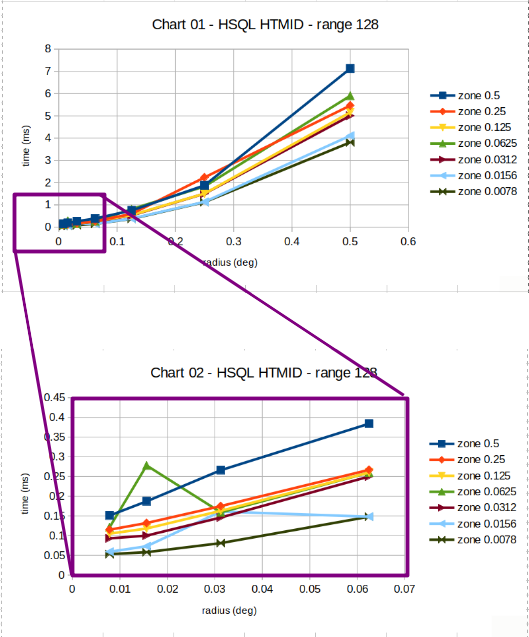
\includegraphics[scale=0.75]{images/graph-zoom-01.png}
\caption{Magnified graph}
\label{fig:graph-zoom-01}
\end{figure}

\subsection{Target speed}
\label{target-speed}

The main aim of these tests was to see if we could find an algorithm and \crossmatch implementation that could meet the required performance target of matching a stream of point sources against a multi-million row \dataset in less than one millisecond per match.

The test results show that the \htmid, zone indexed database implementations and the \cqengine implementation are all capable of reaching this target for a range of values for \dataset size, data density and \crossmatch radius.

\subsection{Algorithm comparison}
\label{algorithm-comparison}

To compare just the \crossmatch algorithms, and to keep as much of the rest of the variables the same, we compared the best set of results for the zone indexed \hsqldb database with the results from the \htmid indexed \hsqldb database.

The results of our tests suggest that in all of the cases we tested the \htmid indexing performed better than the zone based indexing.

Table 01 contains the results for \htmid indexed data:

\begin{table}[hbt!]
\centering
\begin{tabular}{|l|l|l|l|}
\hline
\textit{zone (deg)} & \textit{radius (deg)} & \textit{found} & \textit{timeavg (ms)} \\ \hline
\multicolumn{4}{|c|}{....} \\ \hline
\multicolumn{4}{|c|}{....} \\ \hline
0.0078125 & 0.5       & 46 & 3.811 \\ \hline
0.0078125 & 0.25      & 12 & 1.123 \\ \hline
0.0078125 & 0.125     &  3 & 0.371 \\ \hline
0.0078125 & 0.0625    &  1 & 0.148 \\ \hline
0.0078125 & 0.03125   &  1 & 0.081 \\ \hline
0.0078125 & 0.015625  &  1 & 0.058 \\ \hline
0.0078125 & 0.0078125 &  1 & 0.053 \\ \hline
\end{tabular}
\end{table}

For comparison, table 04 shows the corresponding results for zone indexed data:

\begin{table}[hbt!]
\centering
\begin{tabular}{|l|l|l|l|}
\hline
\textit{zone (deg)} & \textit{radius (deg)} & \textit{found} & \textit{timeavg (ms)} \\ \hline
\multicolumn{4}{|c|}{....} \\ \hline
\multicolumn{4}{|c|}{....} \\ \hline
0.0078125 & 0.5       & 49 & 13.861 \\ \hline
0.0078125 & 0.25      & 10 &  7.499 \\ \hline
0.0078125 & 0.125     &  2 &  3.681 \\ \hline
0.0078125 & 0.0625    &  1 &  1.491 \\ \hline
0.0078125 & 0.03125   &  1 &  1.221 \\ \hline
0.0078125 & 0.015625  &  1 &  0.715 \\ \hline
0.0078125 & 0.0078125 &  1 &  0.424 \\ \hline
\end{tabular}
\end{table}

This shows a clear advantage to the \htmid indexed database compared to the zone indexed database.
This performance difference was observed consistently across all of the cases that we tested, which does not match the results described by Gray et al in 2004\cite{Gray-2004} and Petar Zečević et al in 2019\cite{Zecevic-2019}.

The original goal of our project was to identify a \crossmatch
implementation that was capable of meeting the performance targets, and so the test framework and test data were designed to to look for a specific result, \crossmatching a fix set of data within a specific time.

The \benchmarking comparison between different algorithms and implementations came later as the project evolved. As a result it is likely that our results have been skewed by a systematic error in either our \crossmatch implementation or the generated data used to test them.

It is important to note that where the original papers reported results based on matching real archive data whereas our results are based on generated test data.
The next step would be to run these tests again using data from a real science catalog and compare the results with the results from the generated test data.

We hope to be able to return to these experiments in subsequent projects to improve the accuracy and confidence level of these results.

\subsection{Zone indexing}
\label{zone-indexing}

One aspect of the tests looked at the database query and indexing used in the zone based algorithm.

The SQL query used for the tests came from the query outlined in the paper by Gray et al, which included all three steps in the same query. The initial selection for the target Zone based on declination, the selection within the zone based on right ascension, and then a final selection based on distance.

\begin{lstlisting}[style=SQL]
    SELECT
        ...
    FROM
        zones
    WHERE
        zone BETWEEN ? AND ?
    AND
        ra BETWEEN ? AND ?
    AND
        dec BETWEEN ? AND ?
    AND
        (power((cx - ?), 2) + power((cy - ?), 2) + power(cz - ?, 2)) < ?
\end{lstlisting}

The tests evaluated three different indexing schemes, the first scheme created three separate indexes, one index on the integer zone id, one on the right ascension and one on the declination.

\begin{lstlisting}[style=SQL]
    CREATE INDEX zoneindex ON zones (zone)
    CREATE INDEX raindex   ON zones (ra)
    CREATE INDEX decindex  ON zones (dec)
\end{lstlisting}

The second scheme created two separate indexes, one index for the integer zone id alone, and one index on the right ascension and declination combined.

\begin{lstlisting}[style=SQL]
    CREATE INDEX zoneindex  ON zones (zone)
    CREATE INDEX radecindex ON zones (ra, dec)
\end{lstlisting}

The third scheme created a complex index of zone id, right ascension and declination combined.

\begin{lstlisting}[style=SQL]
    CREATE INDEX complexindex ON zones (zone, ra, dec)
\end{lstlisting}

The results of the tests show a progression based on the zone height. The data in table 31 shows that for a relatively large zone height of 0.5 there is a clear advantage to both the COMBINED and COMPLEX indexing compared to the SEPARATE index.

\begin{table}[hbt!]
\centering
\begin{tabular}{|l|l|l|l|}
\hline
\textit{indexing} & \textit{radius (deg)} & \textit{found} & \textit{timeavg (ms)} \\ \hline
SEPARATE & 0.5 & 50 & 39.47 \\ \hline
SEPARATE & 0.125 & 4 & 20.872 \\ \hline
SEPARATE & 0.03125 & 1 & 21.042 \\ \hline
SEPARATE & 0.0078125 & 1 & 20.545 \\ \hline
COMBINED & 0.5 & 53 & 22.384 \\ \hline
COMBINED & 0.125 & 2 & 14.241 \\ \hline
COMBINED & 0.03125 & 1 & 12.311 \\ \hline
COMBINED & 0.0078125 & 1 & 12.566 \\ \hline
COMPLEX  & 0.5 & 51 & 22.334 \\ \hline
COMPLEX  & 0.125 & 2 & 14.496 \\ \hline
COMPLEX  & 0.03125 & 1 & 13.288 \\ \hline
COMPLEX  & 0.0078125 & 1 & 12.11 \\ \hline
\end{tabular}
\end{table}

However, this advantage gradually becomes less significant as the zone size reduces to the point where the data in table 34 shows that for a zone height of 0.0078125 there is no difference between the three indexing schemes.

\begin{table}[hbt!]
\centering
\begin{tabular}{|l|l|l|l|}
\hline
\textit{indexing} & \textit{radius (deg)} & \textit{found} & \textit{timeavg (ms)} \\ \hline
\multicolumn{4}{|c|}{....} \\ \hline
\multicolumn{4}{|c|}{....} \\ \hline
SEPARATE & 0.5 & 49 & 13.861 \\ \hline
SEPARATE & 0.125 & 2 & 3.681 \\ \hline
SEPARATE & 0.03125 & 1 & 1.221 \\ \hline
SEPARATE & 0.0078125 & 1 & 0.424 \\ \hline
COMBINED & 0.5 & 51 & 14.322 \\ \hline
COMBINED & 0.125 & 3 & 3.143 \\ \hline
COMBINED & 0.03125 & 1 & 1.014 \\ \hline
COMBINED & 0.0078125 & 1 & 0.337 \\ \hline
COMPLEX & 0.5 & 50 & 15.574 \\ \hline
COMPLEX & 0.125 & 3 & 3.335 \\ \hline
COMPLEX & 0.03125 & 1 & 1.093 \\ \hline
COMPLEX & 0.0078125 & 1 & 0.424 \\ \hline
\end{tabular}
\end{table}

This makes sense if we consider the effect of zone height on the number of zones and the count of points within each zone.
As the zone height gets smaller, the data is split across many more zones, which means the index on zoneid is becomes more significant. At the same time, as the zones get smaller, the number of points within each zone get smaller, reducing the significance of the ra and dec indexes within each zone.

\subsection{CQEngine implementation}
\label{cqengine-implementation}

We also developed a native Java implementation of the zone algorithm, which compared the performance of the full relational database engine provided by \hsqldb with an implementation using the \cqengine Collection Query Engine\footurl{https://github.com/npgall/cqengine} library to index data in Java Collections.

The zone algorithm was implemented directly in Java using the \cqengine classes to implement an indexed collection of zones:

\begin{lstlisting}[style=Java]
    public class ZoneMatcherImpl
    implements ZoneMatcher
        {
        ....
        private final IndexedCollection<ZoneImpl> zones =
            new ConcurrentIndexedCollection<ZoneImpl>();
        ....
        }
\end{lstlisting}

and an indexed collection of positions within each zone:

\begin{lstlisting}[style=Java]
    public class ZoneImpl
    implements Zone
        {
        ....
        private final IndexedCollection<PositionImpl> positions =
            new ConcurrentIndexedCollection<PositionImpl>();
        ....
        }
\end{lstlisting}

\subsection{Matcher comparison}
\label{cqengine-indexing}

The test results in table 35 show a comparison between the different \texttt{Matcher} implementations.

\begin{table}[hbt!]
\centering
\begin{tabular}{|l|l|l|l|l|l|}
\hline
\textit{matcher} & \textit{index} & \textit{zone} & \textit{radius} & \textit{found} & \textit{timeavg (ms)} \\ \hline
HsqlHtmidMatcher & HTMID     & 0.5       & 0.5       & 48 &  7.127 \\ \hline
HsqlHtmidMatcher & HTMID     & 0.25      & 0.25      &  9 &  2.234 \\ \hline
HsqlHtmidMatcher & HTMID     & 0.125     & 0.125     &  3 &  0.541 \\ \hline
HsqlHtmidMatcher & HTMID     & 0.0625    & 0.0625    &  1 &  0.26 \\ \hline
HsqlHtmidMatcher & HTMID     & 0.03125   & 0.03125   &  1 &  0.146 \\ \hline
HsqlHtmidMatcher & HTMID     & 0.015625  & 0.015625  &  1 &  0.073 \\ \hline
HsqlHtmidMatcher & HTMID     & 0.0078125 & 0.0078125 &  1 &  0.053 \\ \hline
HsqlZoneMatcher  & COMPLEX   & 0.5       & 0.5       & 51 & 22.334 \\ \hline
HsqlZoneMatcher  & COMPLEX   & 0.25      & 0.25      & 11 &  8.902 \\ \hline
HsqlZoneMatcher  & COMPLEX   & 0.125     & 0.125     &  3 &  5.413 \\ \hline
HsqlZoneMatcher	 & COMPLEX   & 0.0625    & 0.0625    &  1 &  2.444 \\ \hline
HsqlZoneMatcher	 & COMPLEX   & 0.03125   & 0.03125   &  1 &  1.115 \\ \hline
HsqlZoneMatcher	 & COMPLEX   & 0.015625  & 0.015625  &  1 &  0.67 \\ \hline
HsqlZoneMatcher	 & COMPLEX   & 0.0078125 & 0.0078125 &  1 &  0.424 \\ \hline
CQZoneMatcher	 & SEPARATE  & 0.5       & 0.5       & 53 &  5.565 \\ \hline
CQZoneMatcher	 & SEPARATE  & 0.25      & 0.25      & 11 &  0.915 \\ \hline
CQZoneMatcher	 & SEPARATE  & 0.125     & 0.125     &  2 &  0.637 \\ \hline
CQZoneMatcher	 & SEPARATE  & 0.0625    & 0.0625    &  1 &  0.424 \\ \hline
CQZoneMatcher	 & SEPARATE  & 0.03125   & 0.03125   &  1 &  0.638 \\ \hline
CQZoneMatcher	 & SEPARATE  & 0.015625  & 0.015625  &  1 &  1.106 \\ \hline
CQZoneMatcher	 & SEPARATE  & 0.0078125 & 0.0078125 &  1 &  1.826 \\ \hline
\end{tabular}
\end{table}

These results show that the \texttt{HsqlHtmidMatcher} and \texttt{CQZoneMatcher} implementations 
perform at a similar speed when compared to the \texttt{HsqlZoneMatcher} implementation which is significantly slower.

The significant difference between the performance of the \texttt{HsqlHtmidMatcher} and \texttt{HsqlZoneMatcher} implementations, when both are being run on the same database platform with the same data, suggests there may be a problem with the way that the \texttt{HsqlZoneMatcher} database is configured.

\subsection{Summary of results}
\label{crossmatch-summary}

Based on the test results, this set of experiments have been able to demonstrate a \crossmatch algorithm that is capable of meeting the target data rate of 1,000 alerts per second for \catalog sizes of the order of 67 million sources. 
There is more that could be done to develop these experiments further, extending the size of the test \dataset, developing a set of tests using real world science data, optimizing the database indexing and exploring the relationship between zone size, search radius and search performance.

There is also more work to do to explore ways to make the system scalable and fault tolerance by distributing the \crossmatch searches over multiple machines.

\section{Stream processing components}
\label{stream-processing-components}

The following section describes some components that could be used to implement the second stage of the architecture design. Providing a framework to support loosely coupled components that consume data from a stream, apply a filter or processing step, and produce a new stream of results.

\subsection{Java interfaces}
\label{component-libraries.java-interfaces}

The alert processing framework was developed using a set of abstract Java classes and interfaces. However, the concepts modelled by these classes should be portable enough to be represented in any object oriented language.

\subsubsection{Processor}
\label{java-interfaces.Processor}

At the core of the alert processing framework is an interface for a class that can process a candidate.

\begin{lstlisting}[style=Java]
    /**
     * Interface for a Candidate processor.
     */
    interface Processor
        {
        /**
         * Process method response codes.
         */
        enum Response {
            PASS,
            DONE
            };

        /**
         * Process a Candidate and return a response code.
         */
        public Response process(Candidate candidate);
        }
\end{lstlisting}

This interface simply defines a \texttt{process()} method that takes a \texttt{Candidate} object as input and
returns a simple response code, either \texttt{PASS} or \texttt{DONE}.

\begin{itemize}
  \item \texttt{PASS} - Continue processing completed, pass the \texttt{Candidate} on to the next step.
  \item \texttt{DONE} - Processing completed, skip any further steps.
\end{itemize}

\subsubsection{Component}
\label{java-interfaces.Component}

The framework also provides a template implementation of a component that can connect to a Kafka service, subscribed to a \kftopic, read alert messages from the \kftopic, \deserz them into Java objects and passes each \texttt{Candidate} object to a \texttt{process()} method.

\begin{lstlisting}[style=Java]
    /**
     * A component template that includes methods for connecting
     * and subscribing to Kafka streams, reading messages and
     * deserializing alert Candidates.
     */
    public class Component
        {
        //
        // Methods for connecting and subscribing to Kafka streams,
        // reading messages and deserializing alert Candidates.
        //

        /**
         * Template method to process a candidate.
         *
         */
        public void process(Candidate candidate)
            {
            //
            // Code to process a Candidate goes here ...
            //
            }
        }
\end{lstlisting}

Extend this further, adding a list of \javaname{Processor} instances and a \texttt{for} loop to iterate through the list, we can define a \javaname{Component} that applies a sequence of \javaplural{Processor} to an input stream of \javaplural{Candidate}.

 \begin{lstlisting}[style=Java]
    /**
     * A component template that includes methods for connecting
     * and subscribing to Kafka streams, reading messages and
     * deserializing alert Candidates.
     */
    public class Component
        {
        //
        // Methods for connecting and subscribing to Kafka streams,
        // reading messages and deserializing alert Candidates.
        //

        /**
         * Initialise our List of Processors.
         */
        public void init()
            {
            }

        /**
         * Our list of Processors.
         */
        private List<Processor> processors =
            new ArrayList<Processor>();

        /**
         * Top level method to process a Candidate.
         */
        public void process(Candidate candidate)
            {
            foreach (Processor processor : this.processors)
                {
                Response response = processor.process(candidate);

                if (DONE == response)
                    {
                    break;
                    }
                }
            }
        }
\end{lstlisting}

\subsubsection{SolarSystemFilter}
\label{java-interfaces.SolarSystemFilter}

To implement a specific alert processor, the end user only has to provide one or more classes that implement the \texttt{Processor} to populate the list. A simple example of a \texttt{Processor} implementation would be a a solar system object filter.

For alerts that correspond to known solar system objects the \ztf alert messages contain information about the corresponding solar system object.

\begin{itemize}
  \item \texttt{ssnamenr} Name of nearest known solar system object if exists within 30 arcsec (from MPC archive).
  \item \texttt{ssdistnr} Distance in arcsec to nearest known solar system object within 30 arcsec.
  \item \texttt{ssmagnr} Magnitude of nearest known solar system object within 30 arcsec (usually V-band from MPC archive).
\end{itemize}

If we assume alerts that correspond to known solar system objects will have the solar system object name set, and alerts that do not correspond to known solar system objects will have a null value, then we can implement a simple \texttt{Processor} that filters alert candidates and selects those that have been matched with a corresponding solar system object.

\begin{lstlisting}[style=Java]
    /**
     * A filter to detect solar system objects.
     */
    class SolarSystemFilter implements Processor
        {
        /**
         * Check the 'ssnamenr' attribute.
         * @return PASS if it is not null.
         */
        public Response process(Candidate candidate)
            {
            if (null != candidate.ssnamenr)
                {
                return PASS;
                }
            else {
                return DONE;
                }
            }
        }
\end{lstlisting}

If we add an instance of this class to the list of \javaname{Processors} in a \javaname{Component}, we create a processor that will only pass on alert candidates that have been associated with a known solar system object.

\begin{lstlisting}[style=Java]
    class MySolarSystemComponent
        extends Component
        {
        /**
         * Initialise our Component.
         */
        public void init()
            {
            // Initialise our list.
            super.init();

            // Add a SolarSystemFilter.
            this.processors.add(
                new SolarSystemFilter()
                );
            }
        }
\end{lstlisting}

The result is a processor component with all the code for connecting and subscribing to \kafka streams, reading messages and deserializing alert candidates, plus a filter that selects solar system objects.

\subsubsection{DatabaseWriter}
\label{java-interfaces.DatabaseWriter}

Using the same interfaces we can also create a \texttt{Processor} class which writes \texttt{Candidate} objects to a database table.

\begin{lstlisting}[style=Java]
    class MyDatabaseWriter implements Processor
        {
        //
        // Code to connect to a database.
        //

        /**
         * Write the Candidate to a database table.
         * @return Always returns PASS.
         */
        public Response process(Candidate candidate)
            {
            //
            // Code to write a Candidate(s) to a database table.
            //
            return PASS;
            }
        }
\end{lstlisting}

We can combine these two \javaname{Processors} to create a \javaname{Component} filters out solar system objects from the input stream and writes them to a database table.

\begin{lstlisting}[style=Java]
    class MySolarSystemComponent
        extends Component
        {
        /**
         * Initialise our Component.
         */
        public void init()
            {
            // Initialise our List.
            super.init();

            // Add a SolarSystemFilter.
            this.processors.add(
                new SolarSystemFilter()
                );

            // Add a DatabaseWriter.
            this.processors.add(
                new MyDatabaseWriter(
                    "databasename",
                    "tablename"
                    )
                );
            }
        }
\end{lstlisting}

In practice, the project would provide a basic toolkit of processor classes, including processors to write to a range of different database platforms, processors that write messages to \kafka streams, generate \voevent messages, write to a Slack channel or send emails.

\subsection{Workflow configuration}
\label{workflow-configuration}

It is also possible to provide tools for creating processing components and the processors they contain from a simple configuration file. This would enable end users to combine processor classes from the library to create their own processing chains just by writing a \json or \yaml configuration file.

\subsubsection{Solar system example}
\label{workflow.solar-system}

The following \yaml fragment defines a processing component based on the \texttt{Component} described above with an extended version of the \texttt{SolarSystemFilter} that selects alerts associated with named solar system objects, and writes them to a \mariadb database.

\begin{lstlisting}[language=yaml]
  component:
    type: "processing-node"
      params:
        - kafkaurl: "kafka-head:9092"
          topicid: "ztf-buffer"
          groupid: "groupid-f2542d11-1872bee0c055"

      processors:

        filter:
          class:
            "uk.org.example.SolarSystemFilter"
          params:
            - action: "include"
            - targets:
              - "saturn"
              - "jupiter"

        writer:
          class:
            "uk.org.example.MariaDBWriter"
          params:
            - tablename: "ztfevents"
              database:  "jdbc:mariadb://hostname:3306/dbname"
              username:  "Albert"
              password:  "Saxe-Coburg-Saalfeld"
\end{lstlisting}

The component designer creates this \yaml configuration file, or uses a GUI design tool that creates \yaml configuration files like this, and submits it to the system.
The framework behind would create the processing component wrapped up as a \docker container and pass it to the orchestration layer to run one or more instances of it in parallel.

This is a deliberately simplified example, and there are many more details to add, including user accounts, permissions and access controls to limit who is allowed to connect to which streams, who is allowed to create new streams, and what compute resources they are allowed to use, etc.
However, this example is enough to demonstrate the ideas behind a basic framework which enables project developers, and potentially end users, to create alert processing pipelines from a toolkit of building blocks provided by the project.

\subsubsection{Lasair ingestion}
\label{workflow.lasair-ingestion}

Based on this design we can imagine a number of building blocks that could be used to implement parts of the \lasair ingestion process.

Our example list of low speed processors could all be implemented as processing components wrapped up in \docker containers, subscribed to the \stageone input buffer.

\begin{itemize}
  \item Read \avro messages and write them to \avro files for backup.
  \begin{itemize}
    \item Implemented as a \texttt{Processor} that serializes \texttt{Candidate} data to \avro files.
  \end{itemize}

  \item Read alert messages and write candidates to \parquet files analysis using \spark.
  \begin{itemize}
    \item Implemented as a \texttt{Processor} that serializes \texttt{Candidate} data to \parquet files.
  \end{itemize}

  \item Read alert messages, extract the light curves and write them to \fits or \votable files.
  \begin{itemize}
    \item Implemented as a \texttt{Processor} that extracts light curve data from the \texttt{Candidate} and serializes it to a \fits file.
  \end{itemize}

  \item Read alert messages, extract the images and write them to \fits, \png or \jpeg files.
  
  \begin{itemize}
    \item Implemented as a \texttt{Processor} that extracts the images from the \texttt{Candidate} and serialises them to a variety of image formats.
  \end{itemize}
\end{itemize}

Using the proposed architecture, all of these could be described using the \yaml configuration file format, deployed automatically and managed by our orchestration system.

We have already discussed how to implement a filter that selects \texttt{Candidates} that are associated with known solar system objects. This filter could be combined with different database writers to build a set of components that write data about solar system objects to different storage databases.

\begin{itemize}
    \item A \texttt{Component} that selects \texttt{Candidates} that are associated with solar system objects and writes them to a \mariadb database:
    \begin{itemize}
        \item \texttt{SolarSystemFilter} configured to include any solar system object.
    \end{itemize}
    \begin{itemize}
        \item \texttt{MariaDBWriter} writes solar system alerts in a \mariadb database.
    \end{itemize}
\end{itemize}

\begin{itemize}
    \item A \texttt{Component} that selects \texttt{Candidates} that are associated with solar system objects and writes them to a \cassandra database:
    \begin{itemize}
        \item \texttt{SolarSystemFilter} configured to include any solar system object.
    \end{itemize}
    \begin{itemize}
        \item \texttt{CassandraWriter} writes solar system alerts in a \cassandra database.
    \end{itemize}
\end{itemize}

If we create a \texttt{Processor} capable of writing data to a new \kafka stream, we can combine this with our \texttt{SolarSystemFilter} to create a component that reads messages from the \stageone input buffer, selects alert messages associated with known solar system objects and writes them to a new \kafka stream.

\begin{itemize}
    \item A \texttt{Component} that generates a new stream of \texttt{Candidates} that are associated with solar system objects:
    \begin{itemize}
        \item \texttt{SolarSystemFilter} configured to include any solar system object.
    \end{itemize}
    \begin{itemize}
        \item \texttt{KafkaProducer} writes solar system alerts to a new \kafka stream.
    \end{itemize}
\end{itemize}

By extending the \texttt{SolarSystemFilter} to add a switch that either includes or excludes solar system \texttt{Candidates} we could create a component that generates a stream of \texttt{Candidates} that are not associated with any known solar system object.

\begin{itemize}
    \item A \texttt{Component} that generates a new stream of \texttt{Candidates} that are \textbf{not} associated with solar system objects:
    \begin{itemize}
        \item \texttt{SolarSystemFilter} configured to exclude any solar system object.
    \end{itemize}
    \begin{itemize}
        \item \texttt{KafkaProducer} writes solar system alerts to a new \kafka stream.
    \end{itemize}
\end{itemize}

\subsubsection{Crossmatch component}
\label{workflow.cross-match}

Section \ref{crossmatch-algorithms} describes two \crossmatch algorithms for matching alert Candidates against a \catalog of positions.

These \crossmatch algorithms can be used to build a \javaname{CatalogMatcher} component that matches each candidate against a \catalog of positions, adding an annotation to the \javaname{Candidate} object with the result of each match.

Each annotation contains an identifier and position for the \javaname{Candidate}, an identifier and position for the \catalog entry it has been matched with and the distance between the two positions.

\begin{lstlisting}[style=Java]
    interface CandidateMatch
        {
        // Candidate position.
        long   candid();
        double candra();
        double canddec();

        // Catalog position.
        long   catalogid();
        long   sourceid();
        double sourcera();
        double sourcedec();

        double distance();
        }
\end{lstlisting}

We can extend the \javaname{Candidate} class, adding a list of \crossmatch matches, creating a new class, \javaname{AnnotatedCandidate}.

\begin{lstlisting}[style=Java]
    interface AnnotatedCandidate extends Candidate
        {
        List<CandidateMatch> matches();
        }
\end{lstlisting}

We can use this to build a component that combines a \javaname{CatalogMatcher} that matches the candidates against a \catalog and a \javaname{KafkaProducer} that sends the results to a new \kftopic.

In most cases it does not make sense to \crossmatch candidates that have already been associated with known solar system objects, so we want to exclude the solar system objects from the \crossmatch processing.

One way to achieve this would be to use separate \javaplural{Component} and connect them together using \kafka \kfstreams. Connecting the output from a \javaname{SolarSystemFilter} \javaname{Component} to the input of a \javaname{CrossmatchComponent}.

Alternatively, we could combine the \javaname{SolarSystemFilter} and \javaname{CatalogMatcher} in the same \javaname{Component}.

In this example, the resource cost of the \javaname{SolarSystemFilter} is so low, the combined solution is probably the most practical. The resource cost of publishing the non- solar system alerts as a separate \kftopic and reading them back in to the \crossmatch processor out-weighs the minimal cost of including an additional copy of the \javaname{SolarSystemFilter}.

In contrast, a \javaname{CrossmatchProcessor} for a large \catalog requires a lot of resources to implement; significantly more resources than would be needed to handle a new \kftopic in our \kafka \kfbroker. So if we have multiple use cases that need to use the results of the \crossmatch, it would be better to do the \crossmatch calculation once and publish the results as a new \kafka \kftopic for everyone to use.

The cost/benefit of combining \javaplural{Processor} within a complex \javaname{Component}, or deploying them as separate \javaplural{Component} depends on the cost of performing each of the processing steps compared to the cost of publishing a new \kftopic in our \kafka \kfbroker.

High cost processors like the \javaname{CrossmatchProcessor} are a better fit for deploying as separate \kftopics. Low cost processors like the \javaname{SolarSystemFilter} are better suited to being combined into compound \javaname{Components}.

We expect that the science use cases will require a combination of both methods for combining \javaplural{Component} and \javaplural{Processor}, complex \javaplural{Component} and \kftopics.

\subsubsection{Kafka components}
\label{workflow.kafka-components}

There are two options for handling the \kafka \kfstreams and \kftopics needed to link the input and outputs of our \javaplural{Component}. 

The first option is to simply add another \kftopic to the existing \kafka \kfbroker that is providing the \stageone input buffer. However this may cause issues with resource contention for the physical network and storage.
There may be a large number of \kfconsumers subscribed to both the main \stageone \kfbroker \kftopic and the \catalog \crossmatch \kftopics.
In which case it may be better to use a different \kfbroker to provide the internal \kftopics linking the workflow \javaplural{Component}.

Extending this idea further.
If we intend to allow end users to configure their own workflows, then it may make sense to deploy multiple \kafka \kfbrokers, one for each workflow.
To help configure and manage this interconnected network we can treat the \kafka \kfbrokers as just another component, configured and deployed automatically using a similar \yaml configuration file as the processing components.

%\begin{lstlisting}[]
\begin{lstlisting}[language=yaml]
  component:
    type: "kafka-broker"
    servers: 4 
    brokerid: "brokerid-903a2730-240426063766"

    topics:

      - topic:
        - topicid: "topicid-c22d9283-11da68c07e00"
          replication :  1
          partitions  : 64

      - topic:
        - topicid: "topicid-6b5e41ac-c3b83507f47c"
          replication :  1
          partitions  : 64
\end{lstlisting}

This simple \yaml configuration would deploy a new \kafka \kfbroker service, consisting of four \kafka nodes along with the associated \zookeeper service and the monitoring and management services needed to administer them.

Treating a \kafka \kfbroker as just another component makes it easy to deploy it alongside the processing components. A single \yaml configuration file could describe a chain of \kafka \kfbrokers and processing nodes that work together to implement everything needed for a science use case.

Readers familiar with \docker and \kubernetes will recognise a similarity between these \yaml configuration files, \dockercompose configuration files and \kubernetes templates.
Implementing the system behind this framework will probably use many of the infrastructure orchestration tools provided by \openstack, \docker and \kubernetes.
However, where possible we should avoid exposing the implementation details of
these lower level orchestration tools to either our science users or system administrators. The abstract component configuration outlined above is deliberately intended to separate the programming interface that the user interacts with from the orchestration technologies selected to implement the system.

We do not want to develop a new set of orchestration tools. Equally, we do not want implementation specific details of the underlying technologies to be exposed as part of the user interface (GUI or API).

Designing our own abstraction layer has a number of advantages:

1) It provides a level of insulation between our users and the technologies we have selected to build the system. Containerization and container orchestration is a rapidly changing field and the technologies behind it are themselves evolving rapidly.
Using our own components for the user facing interface means we can evolve our implementation to adopt new technologies as they become available without causing migration problems for our users.

2) It is unlikely that one technology will provide everything we will need to implement all of the functionality we want to have. As a result we will need to use a combination of different technologies, tools and frameworks to implement the system. Each of which will have their own programming interface and configuration file syntax.
Using our own components for the user facing API will provide a consistent programming interface and configuration syntax across all the different layers of the system.

3) If we use the same orchestration tool for both the workflow management and the underlying system deployment, then we may run into access control issues.
We do not want our end users to be able to access or modify the deployment of the underlying system services. Which means we would need to implement some form of access control that limits which parts of the system different users are allowed to access and to modify.
If we use our own components for the user facing API, then we can control which parts of the system they have access to. Science users would be able to access and modify their own workflows through the science workflow interface, and system administrators would be able to access the system service deployments using the lower level orchestration tools directly.

4) Using a mapping between our component configuration interface and the underlying technologies means it will be easier to make our components portable across a range of different platforms.

Ideally we would want a researcher to be able to experiment with developing their workflow components on their desktop or laptop, and then be able to deploy the same workflow onto a cloud compute platform without having to make any code changes.

\subsubsection{Updates}
\label{workflow.updates}

The original experiments were done in 2018, and the main text of this report was written in 2019. 
Updating this in 2020 we know a lot more about several of the deployment and orchestration tools that are available.
We expect that \ansible, \terraform and \kubernetes will all play a pivotal role in the development of the platform.
All three of them, to different extents, describe systems in a declarative way.
\terraform and \kubernetes in particular both employ YAML documents that describe the required state of the system and leave it up to the tools to figure out how to implement it.

Everything we have learned since the original set of experiments were performed only strengthens the case for developing a declarative syntax for describing the system and an orchestration framework that builds the system by connecting together ready built components.

\section{Kafka experiments}
\label{kafka-compendium}

This section reports on lessons learned from our experience of working with \kafka during \phasea of the \lsstuk project.

\subsection{Kafka broker}
\label{kafka-broker}

\kafka is a reliable message distribution service for sequential streams of data.

\kafka systems are described in terms of three components, \kfproducers which produce messages, \kfconsumers that consumes messages and a \kfbroker that acts as the store and forward delivery system, accepting messages from \kfproducers and delivering messages to \kfconsumers.

In this scenario, \kafka is the service in the middle, the \kfbroker that provides the message delivery system. The \kfproducer and \kfconsumer are clients, external and separate from the \kafka \kfbroker.

The \kafka \kfbroker does not know where the messages come from, or what happens to them after they are delivered.
The \kafka \kfbroker concentrates purely on listening for messages from \kfproducers, storing them in a buffer and forwarding them on to \kfconsumers.

\subsection{Publish-subscribe pattern}
\label{kafka-pubsub-pattern}

This separation between the delivery system and the message producing and consuming clients is referred to as the publish-subscribe or 'pub-sub' pattern\footurl{https://en.wikipedia.org/wiki/Publish-subscribe_pattern}.

The publishing component of the publish-subscribe pattern is referred to as a \kfpublisher.

In the publish-subscribe pattern, a \kfpublisher does not send the messages directly to their final destination. Instead the messages are tagged as belonging to a \kftopic and sent to the \kfbroker.
Once a message has been sent to the \kfbroker the \kfproducer is no longer involved in the delivery.

The \kfpublisher does not need to know anything about the \kfsubscribers, how many there are, where they are or what they do with the messages.
The \kfbroker is responsible for storing and forwarding the message to the correct destinations, leaving the \kfproducer free to work on producing the next message.

The subscribing component of the publish-subscribe pattern is referred to as a \kfsubscriber.

A \kfsubscriber does not need to know anything about the \kfpublishers, it just receives messages from the \kfbroker. 
The \kfsubscriber contacts the \kfbroker and asks to subscribe to a \kftopic. The \kfbroker will then pass on any messages it receives that have been tagged as belonging to that \kftopic.

The choice of which messages belong to which \kftopics is not made by the \kfbroker. The assignment of messages to \kftopics is made by the \kfpublisher when it sends message to the \kfbroker.
The \kfbroker does not read, interpret or filter the messages. It just passes messages on to \kfsubscribers based on which \kftopics the messages were tagged with. 

\subsection{Producers and consumers}
\label{kafka-producer-consumer}

In \kafka terminology the \kfpublisher component of the publish-subscribe pattern is called a \kfproducer, and a \kfsubscriber component is called a \kfconsumer.

At the implementation level, a \kfpublisher uses a connector class from the \kafka client library to send messages to a \kafka \kfbroker.
The connector class in the client library also called a \javaname{Producer}.
In terms of what is in the program source code, a message \kfpublisher sends its messages by calling the \javaname{write()} method on a \javaname{Producer} object.
This quirk of naming can cause some confusion when talking about \kfproducers and \kfconsumers.
It is important to keep in mind that the class in the client library is not a \kfproducer, it does not produce messages, it is just a connector. The whole message generating component is the \kfproducer, which uses an instance of a connector \javaname{class} from the \kafka client library to send messages to the \kfbroker.

Similarly on the receiving side, a \kfsubscriber, or \kafka \kfconsumer, uses a connector class from the \kafka client library to receive messages from a \kafka broker.
The class in the client library that reads messages from a broker is also called a \javaname{Consumer}. In terms of what is in the program source code, a message \kfsubscriber receives messages by calling the \javaname{read()} method on a \javaname{Consumer} object.
Again it is important to keep in mind that the class in the client library is not a \kfconsumer, it is just a connector. The whole message handling component is the \kfconsumer, which uses an instance of a connector \javaname{class} from the \kafka client library to receive messages from a \kfbroker.

\subsection{Avro encoding}
\label{avro-encoding}

As far as the \kafka \kfbroker is concerned, the content of the messages is opaque. The \kafka \kfbroker does not look at the content of messages, it just delivers them.
The \kfbroker handles messages as simple arrays of bytes, regardless of their content.

A common pattern is to use the  \avro serialization format to encode messages handled by \kafka.
There are strong links between the \kafka and \avro development 
communities and developers from \confluent \footurl{https://www.confluent.io/} contribute to the development of both projects.
However using one does not require the use of the other.

\begin{itemize}
    \item \avro is a binary serialization encoding used by many different applications.
    \item \kafka is a publish-subscribe message broker that handles messages in any format, irrespective of how the message content is encoded.
\end{itemize}

\subsection{Avro schema}
\label{avro-schema}

Using \avro to encode the message content requires the \kfpublisher and \kfsubscriber to share information about the message \avschema to enable the recipient to decode the binary bytes back into usable message content.

However the \kfbroker itself does not provide any support for sharing metadata about the message \avschema. \kafka is not directly linked to \avro and the \kfbroker cannot see inside the messages. It is up to the system developers to figure out how to share metadata about the message \avschema between \kfproducers and \kfconsumers. 

There are three main patterns used to share information about the message \avschema between \kfproducer and \kfconsumer.

\subsubsection{Static shared schema}
\label{avro-static-schema}

The simplest method is to fix the message \avschema beforehand, giving both \kfproducer and \kfconsumer a static copy of the \avschema.  In this method the  messages are transmitted as-is, as binary arrays, without any additional metadata about the \avschema.

This works for simple test systems, but it is inherently fragile and will break the first time that we add a new  \kfproducer that uses a slightly different \avschema.

There is enough built-in error checking in the \avro serialization encoding for a client to be able to validate a message against a message \avschema. However, the validation process costs a non-trivial amount of compute resources, and in the end all it can produce is a simple PASS/FAIL result to indicate whether the message matches the expected \avschema.

Most implementations that use a shared static \avschema rely on an external, out of band, process to ensure the \kfproducer and \kfconsumer use the correct \avschema. Again, this works for simple test systems, but it is inherently fragile and does not scale to handle multiple different types of messages.

\subsubsection{In-line schema}
\label{avro-inline-schema}

The in-line method embeds the \avschema into the header for each message.
Every message includes a full copy of the message \avschema, serialized as a plain text \json\footurl{https://www.json.org/} document.

This means that all the messages are self-describing. A client does not need to know about the message \avschema beforehand, it can use the embedded \avschema to \deserz a message into a generic structure on the fly.

However, embedding the \avschema in every message adds a non-trivial overhead, particularly if the \kfstream only contains a small number of well known message types.
In the current ZTF \kfstream, every message carries with it a copy of all four \avschema files:

\begin{itemize}
  \item alert.avsc (1094 bytes)
  \item candidate.avsc (14784 bytes)
  \item cutout.avsc (236 bytes)
  \item prv candidate.avsc (6565 bytes)
\end{itemize}

This adds an overhead of 22,679 bytes to every message. Scale that up to the 10kHz data rate expected from LSST and this represents a continuous load of over 220 Mbytes per second to continuously re-transmit the same \avschema information to all of the \kfconsumers.

Sending the \avschema with the message means the message is self-describing, but it also means that the client is encountering the structure for the first time every time it receives a message. If the client is \deserzing messages on the fly using the \avschema from the message header, then the client is unable to apply any form of optimisation to the decoding process. It has to \deserz the message into a generic object structure each time, which can be inefficient to construct and inefficient to use.

The current ZTF message handling uses a combination of both the static \avschema and inline \avschema methods.
The upstream ZTF \kfproducer is sending a full copy of the \avschema in the header of every message, but not all of the clients are making use of this. 
Some of the clients ignore the \avschema in the header and use a \deserzer built from a static copy of the \avschema embedded in the client source code, leaving them vulnerable to changes to the message \avschema from the upstream \kfproducer.

This incorporates the bad parts of both options, the overhead of transmitting a full copy of the \avschema with every message, while still having fragile \kfsubscribers that rely on static copies of the \avschema.

\subsubsection{Schema registry}
\label{avro-schema-registry}

The third option is to use a \conschemareg pattern developed by \confluent which uses a \conschemaregistry to link the message \avschema with a numeric identifier based on a hash of the \avschema content.
This identifier is sent in the message header, replacing the full \avschema with a simple numeric value.

The client software contains a set of compiled \deserzers for known message structures.
These \deserzers are built from static copies of the \avschema and can be optimised to generate fully qualified object classes that directly represent the message structure.

If the upstream \kfproducer produces a message based on one of these known message types, then the client will recognise the \avschema identifier and use it to load the corresponding \deserzer to \deserz the message into an object.

If the upstream message \kfproducer introduces a new type of message, one that is not in the client's library of \avschema, then the client can use the \avschema identifier to resolve the \avschema in the \conschemareg and download a copy of the registered \avschema. 

\confluent have defined a wire protocol  format\footurl{https://docs.confluent.io/current/schema-registry/serdes-develop/index.html#wire-format} for embedding \avschema identifiers at the beginning of a message.

The format starts with a single byte to represent the serialization format version (zero in the current version) followed by four bytes for the \avschema identifier and then the rest of the message body.

\begin{table}[hbt!]
\begin{tabulary}{\linewidth}{|L|L|L|}
\hline
\textit{Byte} & \textit{Field} & \textit{Description} \\
\hline
0 & Magic Byte & Confluent serialization format version number; currently always 0. \\
\hline
1-4 & Schema ID & Four byte schema ID from the \conschemaregistry. \\
\hline
5+ & Data & Serialized data for the specified \avschema format (e.g. binary encoding for Avro or Protocol Buffers). \\
\hline
\end{tabulary}
\end{table}

\confluent also have defined a REST \webservice interface for a \conschemaregistry \footurl{https://www.confluent.io/confluent-schema-registry/}
that provides a standard service API for \kfproducers and \kfconsumers to register and resolve information about message \avschema.

A \kfproducer uploads their message \avschema to the REST service to register it and get a unique numeric identifier in return.
The first time a \kfconsumer encounters a message with a \avschema identifier it does not recognise it can call the \conschemaregistry service to resolve the \avschema identifier and download a copy of the \avschema.

The \kfconsumer can use this downloaded \avschema to create a \deserzer that can \deserz with the message structure.

In effect this is an indirect version of the in-line \avschema pattern. Using the \conschemaregistry to transfer a copy of the message \avschema from the \kfproducer to the \kfconsumer. However, this only has to be done once, when the \kfconsumer first encounters a message with this \avschema identifier. For subsequent messages with the same \avschema identifier, the \kfconsumer can use the local cached copy of the \avschema and corresponding \deserzer.

This reduces the transmission overhead from 22,000 extra bytes to 5 bytes per message, 1 for the \avschema version and 4 bytes for the \avschema identifier. It also means the \kfconsumer does not have to construct a new \deserzer every time, it can re-use a cached \deserzer linked to the \avschema identifier.

This scheme works well to create flexible \kfconsumers that can handle multiple message structures and is used extensively by the \confluent tools and services such as the \confluent Connect\footurl{https://docs.confluent.io/current/connect/index.html} components and \confluent Platform\footurl{https://www.confluent.io/product/confluent-platform} frameworks.

The \conschemaregistry service is designed to manage the \avschema for an entire organisation, including support for deploying a distributed registry service that functions across more than one \datacentre.
However, this pattern does not work for managing \avschema across multiple organisations.

The first problem is that the \avschema identifier is just a single 32 bit integer, assigned by the central registry service for the organisation. This identifier is guaranteed to be unique within the host organisation, but as far as we know there is no way of extending this to span multiple organisations.

The second problem is that the message header only contains the 32 bit numeric identifier, it does not contain any information about \textit{which} \conschemareg service to use to resolve the identifier.
The \conschemaregistry pattern relies on all the \kfproducers and \kfconsumers within an organisation configured with the same endpoint address for the one central \conschemaregistry service; which does not scale to register and resolve \avschema across separate organisations.

If the \kfproducers and \kfconsumers are in different organisations, and using different \conschemaregistry services, then a \kfconsumer has no way of discovering which \conschemareg it should use to resolve the numeric identifier into the corresponding \avschema.

The \confluent system does support deploying a distributed \conschemaregistry across multiple physical \datacentres\footurl{https://docs.confluent.io/current/schema-registry/multidc.html}, by configuring one \conschemareg as the primary and the other \conschemaregs as secondaries.
These secondary \conschemaregs are not able to register new \avschema themselves, they must pass all new \avschema back to the primary \conschemareg for registration, centralising the  generation of identifiers and ensuring they remain unique within the organisation.

Passing new \avschema back to the primary \conschemareg for registration means that while this model may work for \textasciitilde 10 \datacentres within an organization, it is unlikely to scale to include a multi-level hierarchy of \textasciitilde 100 different organizations within the astronomy domain.
If all of the secondary registries are required to register their \avschema with the top level primary registry, then the \lsst project would become the de facto central \conschemaregistry for the entire astronomy domain. 

At the time of writing, the \lsst project had not decided on what methods they would eventually adopt for managing version control for their message \avschema. However a number of their design documents refer to the \confluent \conschemaregistry as a possible solution.

\begin{quote}
\textit{“The LSST Project will make available a registry of all alert schemas ever used operationally by LSST. Schemas may be retrieved from this registry by some convenient interface given a four-byte schema ID. Conceptually, this is equivalent to the Confluent Schema Registry, although it is possible an alternative implementation will be deployed in practice."}\footurl{https://dmtn-093.lsst.io/#management-and-evolution}
\end{quote}

\begin{quote}
\textit{“... we have not committed on a particular mechanism for distributing the alert format and making changes to it. One option is the Confluent Schema Registry [1]; choosing this option may have implications on the deserialization performance of consumers.”}\footurl{https://dmtn-149.lsst.io/#alert-format}
\end{quote}

\subsubsection{Gateway broker}
\label{avro-schema-gateway}

If the \lsst project do adopt the \confluent \conschemaregistry to register their alert \avschema, then the \lsstuk project will need to develop a similar mechanism for managing version control of message \avschema within the \lsstuk project.

The following proposal outlines the design for a gateway \kfbroker that would handle the mapping between \avschema identifiers from the upstream \lsst \conschemaregistry and \avschema identifiers in the local \lsstuk \conschemaregistry.

The first part of the solution is to deploy a local instance of the \confluent \conschemaregistry which would be responsible for managing all the \avschema versions within the \lsstuk organization.

We would then need to create a mapping between \avschema identifiers in messages from the upstream \lsst \kfbroker and the corresponding \avschema identifiers in our own \conschemaregistry.

This could be handled by deploying a modified form of the mirror maker service already in use as part of the \stageone buffer.
This gateway service would maintain a mapping between \avschema identifiers from the upstream \lsst \kfbroker and those in the local \lsstuk \conschemaregistry and translate the \avschema identifiers on the fly as it imported messages from the upstream \lsst \kfbroker into the \lsstuk system.

The gateway service would read the four byte \avschema identifier from each message and check for a corresponding \avschema in the local \conschemaregistry. If it did not find a matching \avschema then it would call the upstream \conschemaregistry provided by \lsst to resolve the \avschema identifier, download a \json encoded copy of the \avschema and then register the new \avschema in the local \conschemaregistry. This would generate a new identifier, valid for the local domain.
The gateway \kfbroker can then replace the four byte \avschema identifier in each message from the upstream \kfbroker with the corresponding local identifier from the local \conschemaregistry before it passes the message on to the \lsstuk \kfbroker system.

Using a gateway \kfbroker like this enables the \lsstuk project to maintain a local \conschemaregistry to provide version control for all of the message \avschema used by the \lsstuk system. This would include copies of \avschema published by the upstream \kfbroker and any internal \avschema generated by dynamic database queries and filtering components within the \lsstuk system.

\subsection{Kafka replication}
\label{kafka-data-storage}

A \kafka server stores data for a topic as a set of log files which are split into \kfpartitions and distributed across the servers in a cluster.

The number of \kfpartitions is set by the client when the topic is created and the \javaname{Producer} class from the client library is responsible for distributing the data across \kfpartitions.

%\begin{figure}[H]
%\centering
%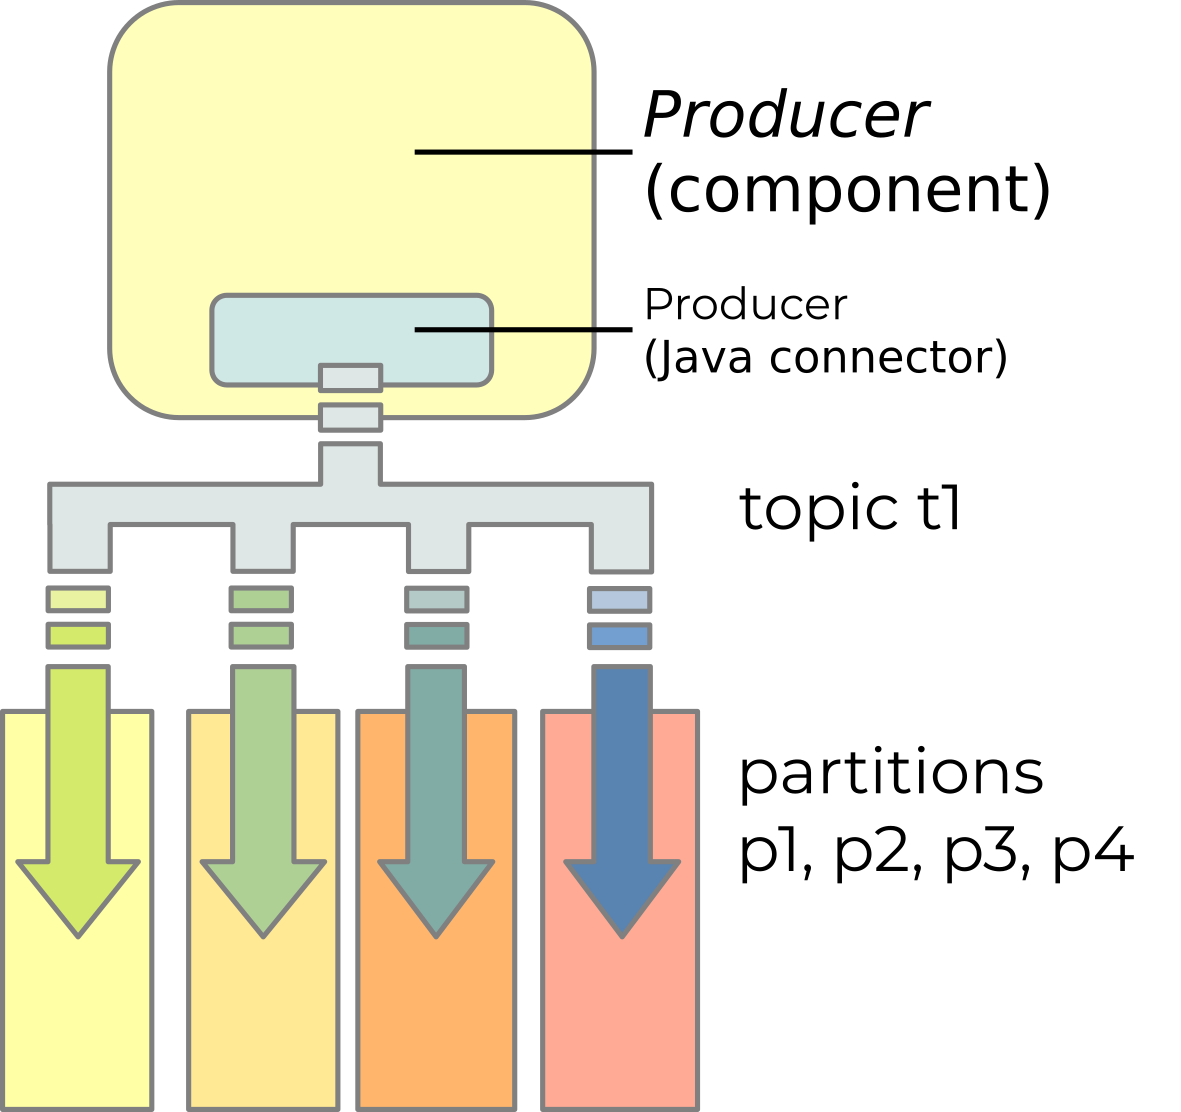
\includegraphics{images/kafka-partitions-01.png}
%\includesvg{images/kafka-partitions-01.svg}
%\caption{Client \javaname{Producer} distributes messages to %\kfpartitions}
%\label{fig:kafka-partitions-01}
%\end{figure}

The total number of log files is set by the number of \kfpartitions multiplied by the replication factor set for that topic.
If a topic has four \kfpartitions, and a replication factor of three, then the data will be spread across 12 log files.
If this topic is served by four servers, then each server will be allocated three of the 12 files.

The \javaname{Producer} client connector writes each \kfpartition to one server. Replicating the data to the other servers in the cluster is handled internally by server to server transfers.

\begin{figure}[H]
\centering
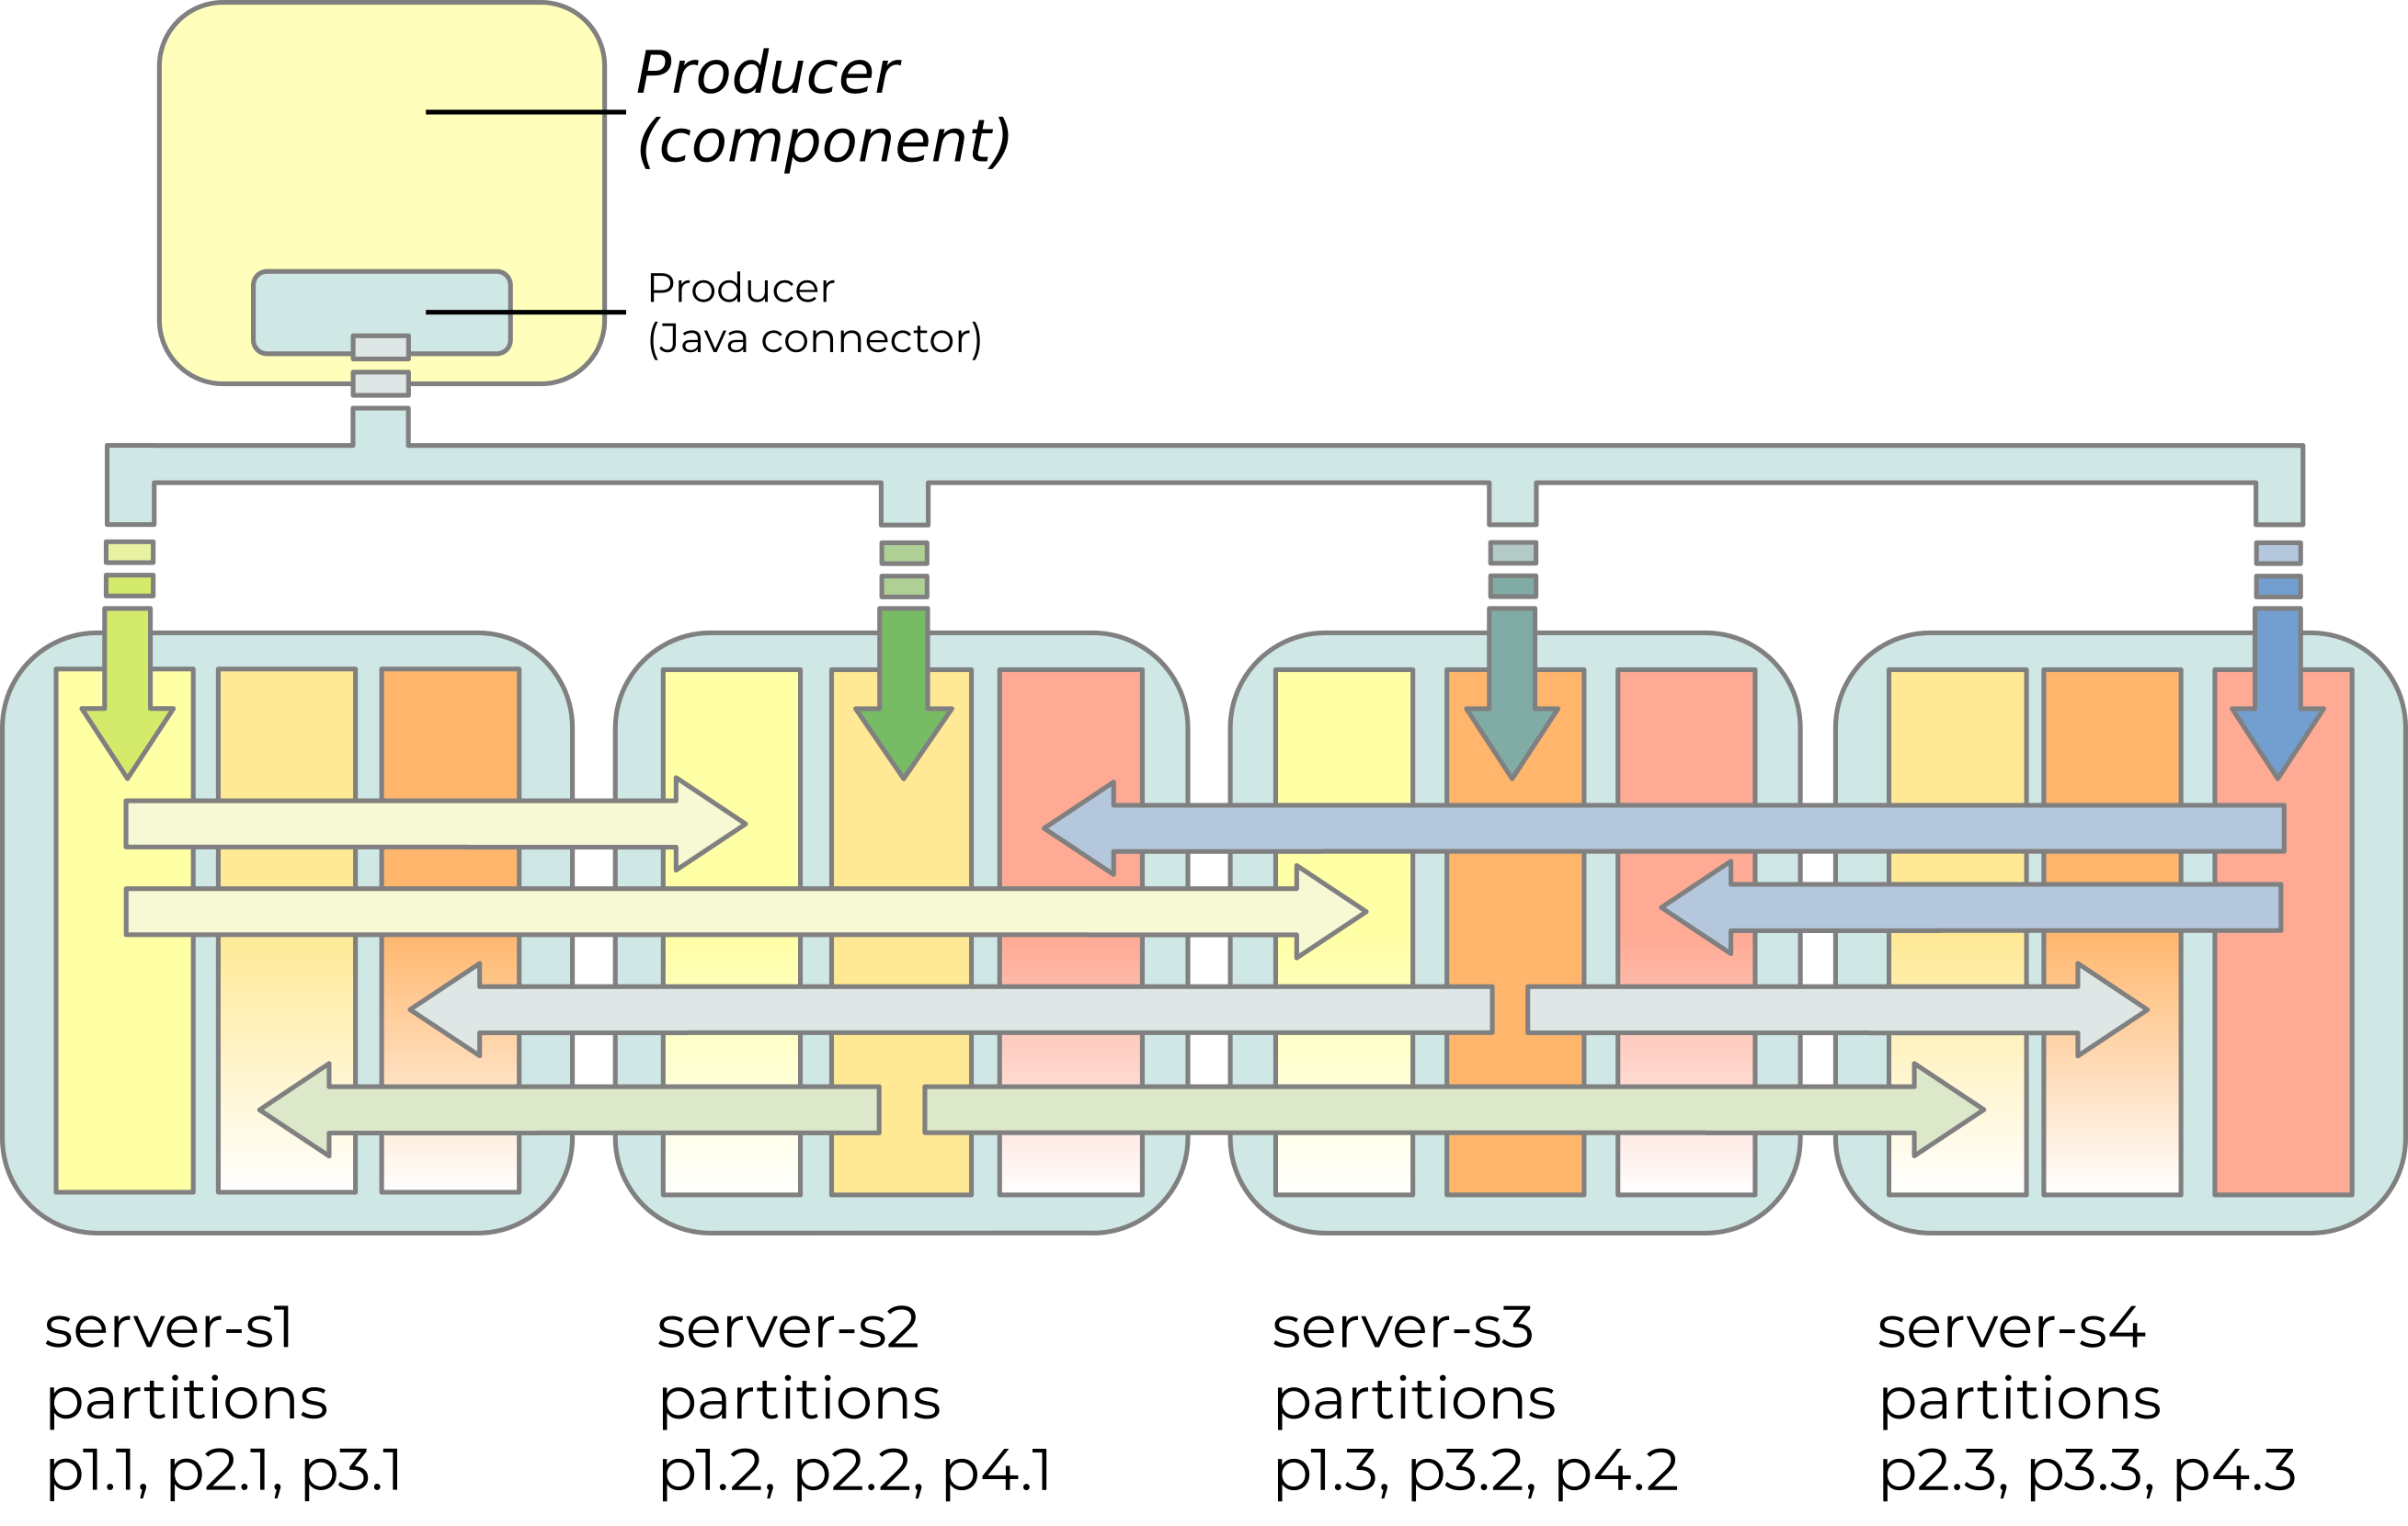
\includegraphics{images/kafka-partitions-03.png}
%\includesvg{images/kafka-partitions-03.svg}
\caption{Client \javaname{Producer} distributes messages to \kfpartitions}
\label{fig:kafka-partitions-03}
\end{figure}

If we lose one of the machines, server-s2 for example, the system still has two copies of each of the three \kfpartition files that were on server-s2.

\begin{itemize}
    \item \kfpartition-p1 is on server-s1 and server-s3
    \item \kfpartition-p2 is on server-s1 and server-s4
    \item \kfpartition-p4 is on server-s3 and server-s4
\end{itemize}

If we replace server-2 with an empty machine, the three missing log files can be recovered using data from the other servers.

\begin{figure}[H]
\centering
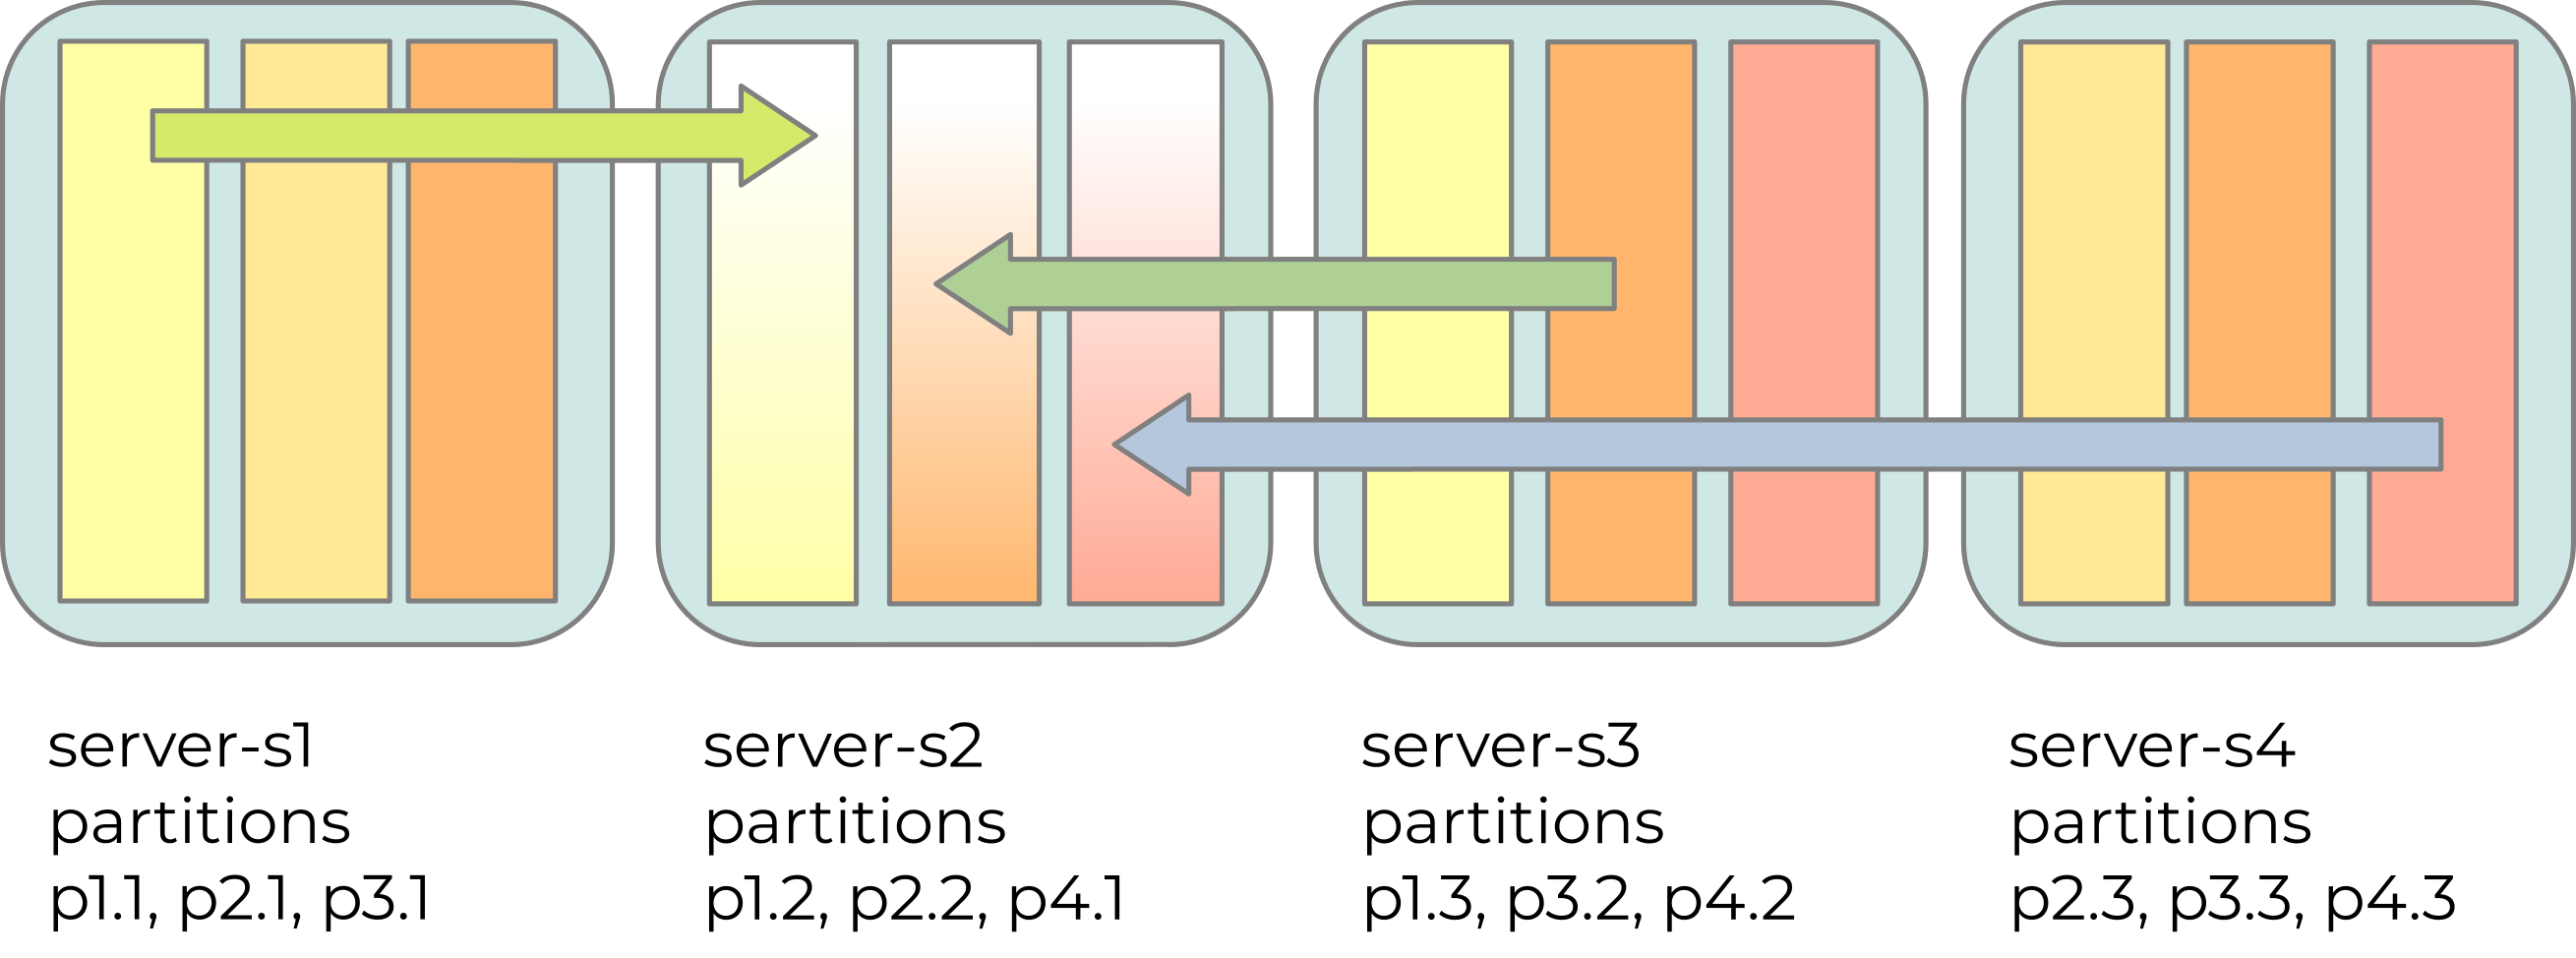
\includegraphics{images/kafka-partitions-04.png}
%\includesvg{images/kafka-partitions-04.svg}
\caption{Missing data recovered from replicas}
\label{fig:kafka-partitions-04}
\end{figure}

Our experience of using \kafka on an unreliable cloud platform that is having issues with virtual machines losing contact and dropping off the network is that the \kafka replication system works well and enables system administrators to provide a reliable and fault tolerant \kfbroker service even when the underlying platform is not reliable.

However, we did encounter a couple of issues that system administrators should be aware of.

\subsubsection{Storage replication}
\label{storage-replication}

If the \kafka system is deployed on an \openstack cloud platform, then a fairly common way to manage storage space for the \kafka nodes is to use the Cinder\footurl{https://docs.openstack.org/cinder/latest/} block storage service to provide virtual discs on each node.

A fairly common way of implementing the Cinder block storage service for an \openstack deployment is to use a \ceph\footurl{https://docs.ceph.com/} service to aggregate storage space across the network to provide a distributed file system for Cinder to use\footurl{https://docs.openstack.org/cinder/pike/configuration/block-storage/drivers/ceph-rbd-volume-driver.html}.

The \ceph service may itself use data replication to improve the reliability of the distributed file system.
As a result, the combination of default configurations may mean that the data is replicated twice. Once by \kafka itself and again by the underlying \ceph service used by \openstack.

This is not always a problem, and in fact using RAID replication for the \ceph distributed file system can improve the performance of the system.

In theory it is possible for \openstack users to control the level of replication that is used for Cinder volumes. However, exposing the volume type configuration options to end users is not necessarily available on all \openstack deployments.

System administrators need to be aware that this is happening and take steps to make sure it is configured correctly. 

Replicating the data multiple times can have cost implications for a large scale deployment, possibly doubling or tripling the cost of storage space.

\subsubsection{Storage validation}
\label{storage-validation}

\kafka is designed to prioritise the integrity and reliability of the cluster.
As part of this, on startup, each \kafka node will validate all of the data in its local directories before it becomes active and joins the cluster.

In most situations, this works well, and ensures that a \kafka node with corrupted data does not join an active cluster and replicate the corrupted data to other nodes.

However, if a \kafka node is storing a lot of historical data or is configured with a high level of replication, then this data validation process can become counter productive.

As part of our experiments with \kafka we configured a \kfbroker to maintain a full history of the \kftopics transmitted from \ztf by setting the retention period and space quotas to zero, preventing the \kfbroker from deleting any of the data it received.
As a result the system gradually accumulates more and more data over time, building a permanent archive of all the daily \kftopics published by \ztf.

This works well while the system is up and running, but may cause problems when the system is shutdown and restarted.

On restart, all of the nodes will validate all of the data in their local directories before they attempt to register as members of the cluster.
This may take a significant amount of time, from several minutes to several hours, depending on the amount of data they have accumulated and how it is stored.

Under normal conditions, while the \kafka \kfbroker is up and running, the nodes only need to access a small quantity of data from disc at any one time. 
Most of the time the \kfbroker nodes will be sequentially writing new blocks to the leading edge of each \kfpartition as new messages arrive and they will try to reduce the amount of random reads from disc by maintaining a buffer of recent data in memory.

On restart, each node has to do a full scan of all the data in their local directories to validate all the replicas of all the \kfpartitions stored on that node.

To make matters worse, on a clean startup of the system, all the nodes are attempting to do this all at the same time. This will place a high load on any resources shared between the nodes.
If the nodes are configured to use a network mounted file system, such as Cinder volumes on an \openstack deployment, then the network infrastructure needs to be able to cope with a sustained high load while all of the nodes validate their data.
If several nodes are configured to share space on the same physical disc then the sustained load of multiple concurrent random reads may have a significant impact on performance.

In a worst case example, one of our experiments had four \kafka nodes sharing space on the same set of physical hard discs. The \kafka \kfbroker was configured to keep a full record of all the messages and had been accumulating data for around six months.
When this service was restarted, the cumulative effect of all four nodes trying to scan all their data at the same time meant the data validation process took more than 20 hours to complete.
During which time, the \kafka \kfbroker had no active nodes in the cluster and was unable to process any new messages.

In this case, this service was deliberately configured this way to learn what would happen.
The \kafka user guide explicitly advises system administrators not to share disc spindles between \kafka nodes for this reason.

Based on our experience with administering a \kafka \kfbroker it is worth experimenting with different "what if" scenarios like this to learn how \kafka behaves when things go wrong and how to manage them when they do.

\subsection{Kafka partitions}
\label{kafka-partitions}

The partitioning and replication of data is essential to the way that Kafka operates, and provides much of its performance and reliability benefits.
However, the choice of how \kftopics are partitioned is not necessarily as simple as first expected and system administrators need to be aware of how it can affect system performance for the \kfbroker itself and for downstream data processing components.

The key issue that needs to be considered is the number of \kfpartitions for each \kftopic. If we consider an example configuration of a \kfproducer connected to a set of four servers.

If the \kftopic is configured to have only three \kfpartitions, the \kfproducer will distribute the data to each of the three \kfpartitions in turn.

The messages are sent to the servers in blocks. The number of messages in each block is determined by the size of the individual messages and the size of the transmit buffers configured on the client and servers.
If we simplify the distribution process to a round-robin selection, then the first block of messages will be sent to \kfpartition 1 on the first server, the second block is sent to \kfpartition 2 on the second server, and the third block is sent to \kfpartition 3 on the third server.

The fourth block of messages are not sent the fourth server because the \kftopic is configured to have only three \kfpartitions.
Instead the fourth block is sent to \kfpartition 1 on the first server, the fifth to \kfpartition 2 on the second server, and so on.

\begin{figure}[H]
\centering
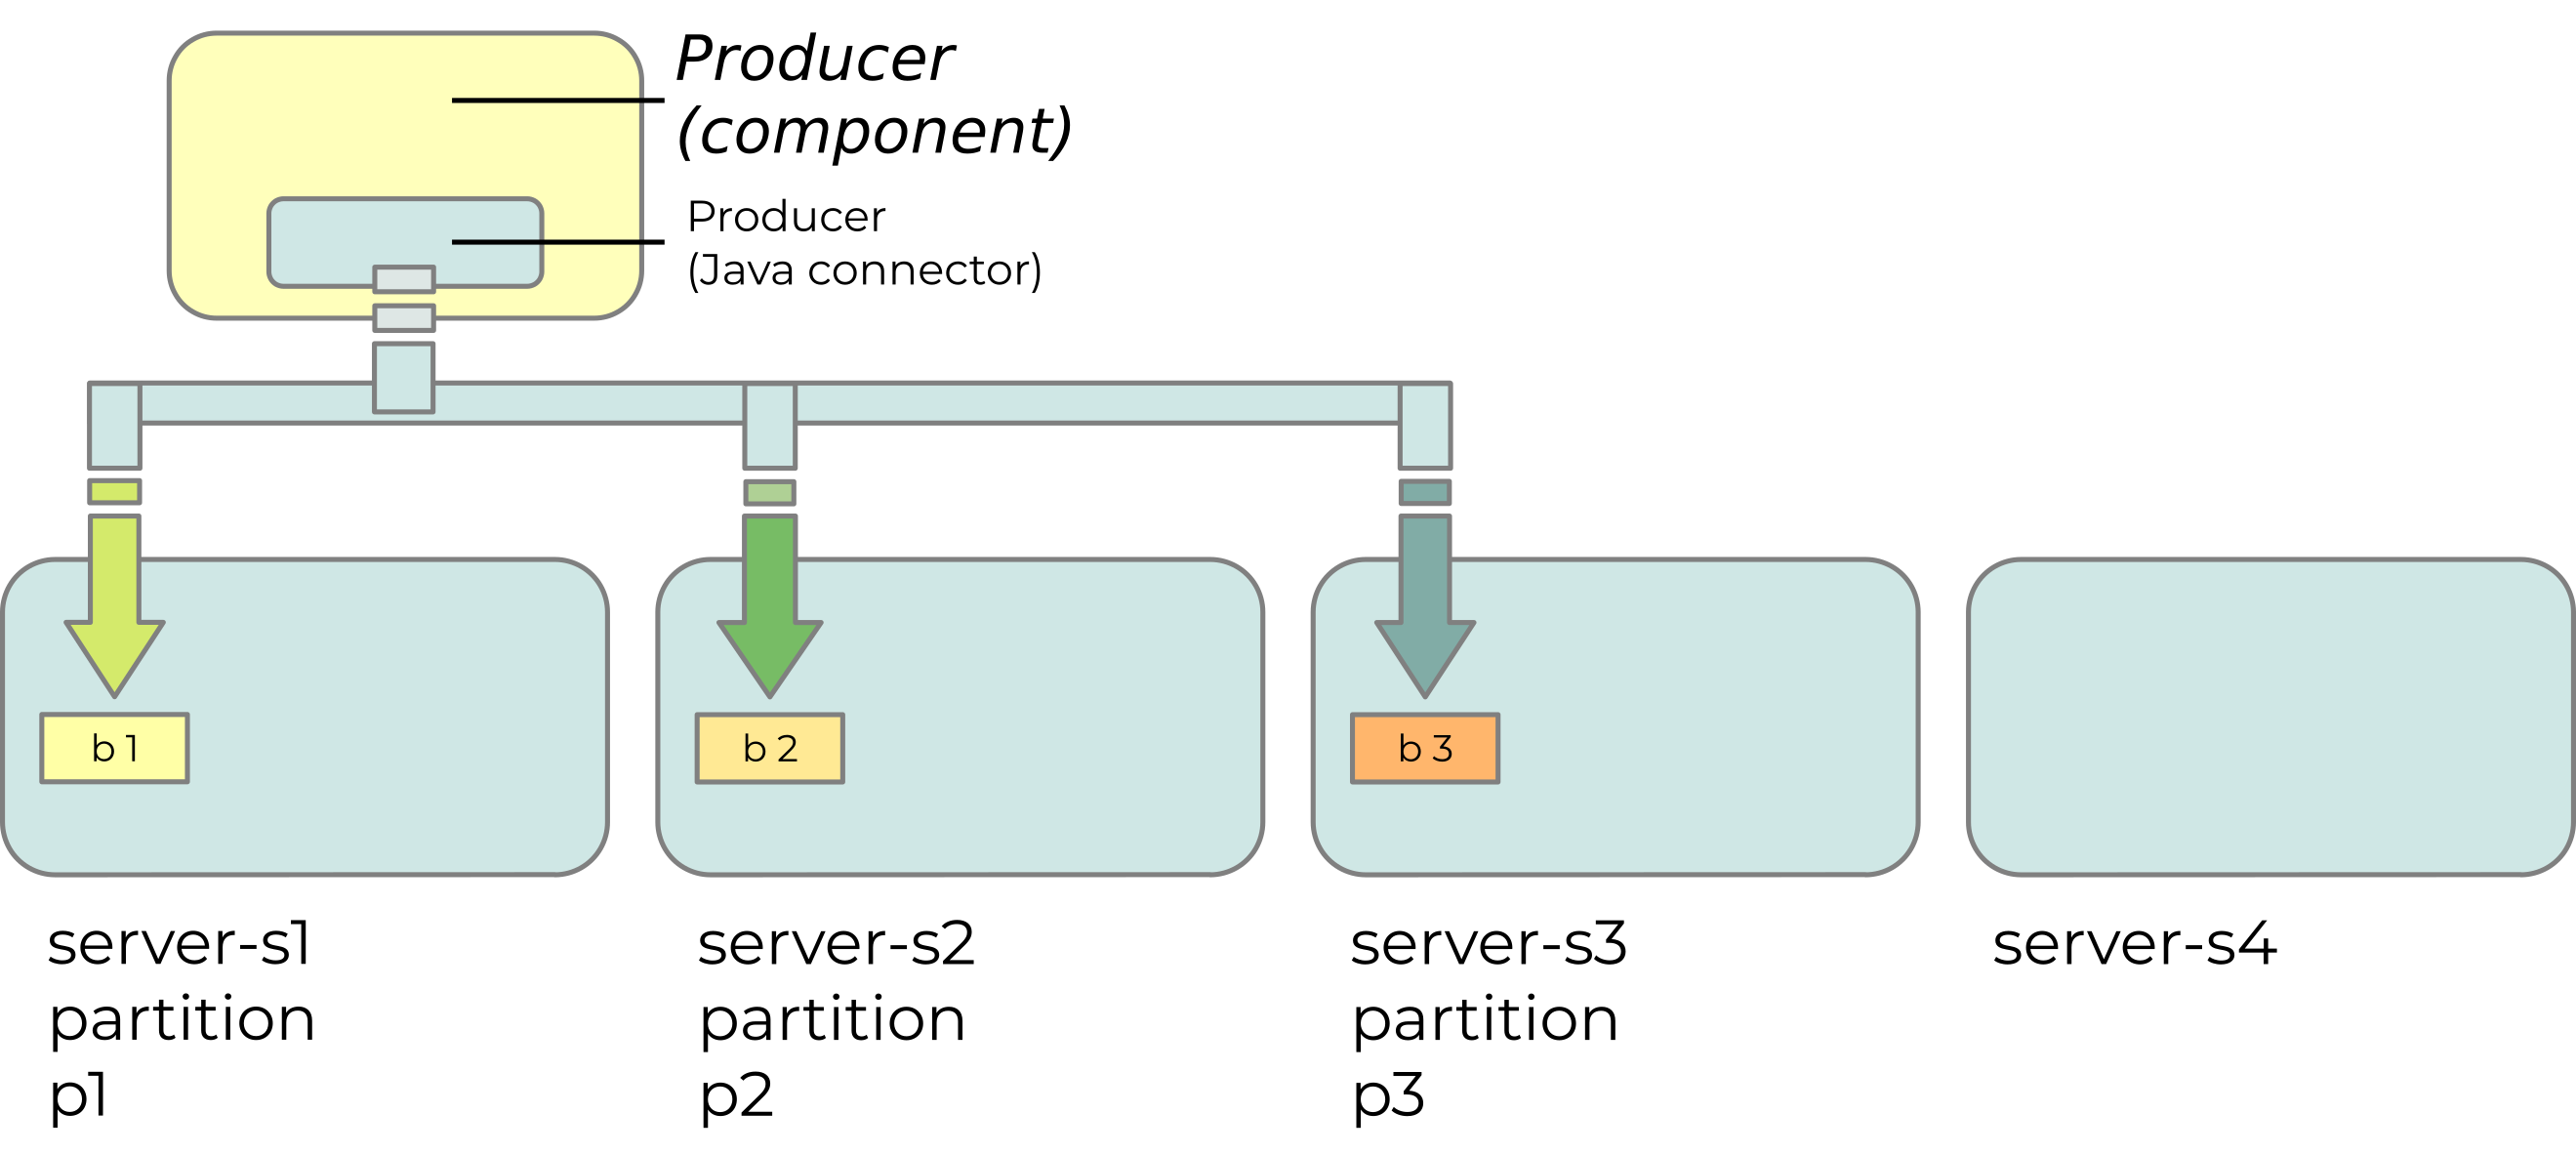
\includegraphics{images/kafka-partitions-05.png}
%\includesvg{images/kafka-partitions-05.svg}
\caption{5 blocks distributed over 3 partitions}
\label{fig:kafka-partitions-05}
\end{figure}

In this configuration, with more nodes than \kfpartitions, the fourth node does not have any \kfpartitions allocated to it.
In reality, the replication factor would normally be greater than one, so internal replication would spread copies of the data between the four nodes, and so the fourth node would get a share of the data.
However, to simplify this example we are only tracking the primary copies for each \kfpartition and not the replicas.

If we increase the \kfpartition count to four, then the \kfpartitions are spread evenly across all four nodes.

If the \kfproducer sends six blocks of messages they are spread as evenly as possible between the four \kfpartitions; \kfpartitions 1 and 2 will get two data blocks each and \kfpartitions 3 and 4 will get just one data block.

With five \kfpartitions, then three of the four nodes would have one \kfpartition each, and one of the nodes would have two \kfpartitions.

With six \kfpartitions, then two of the have two \kfpartitions and two of the servers have one \kfpartition.

As the number of \kfpartitions increases, the data is spread more evenly across the nodes.
With 25 \kfpartitions, three of the four nodes would have six
\kfpartitions, and one of the nodes would have seven \kfpartitions.
The general rule is configuring a \kftopic to have more \kfpartitions will spread the data more evenly across the available resources.

The same process of distributing data between resources applies to \kfconsumers receiving data from the \kfbroker.

Starting with our first example, three \kfpartitions spread across four nodes. If we have a single consumer, then data from all four \kfpartitions are sent to the same consumer.

If we add a second consumer, then one \kfconsumer would receive data for two of the \kfpartitions and one \kfconsumer would receive data for the remaining \kfpartition.
Note that \kafka will not share data from a \kfpartition between \kfconsumers, so it will not allocate one and a half \kfpartitions of data to each of the two \kfconsumers.

If we have three consumers, then each consumer receives data from one \kfpartition.

If we have four consumers, then three of the consumers each get data from a \kfpartition, and the fourth consumer does not receive any data.

Increasing the number of \kfconsumers beyond the number of \kfpartitions results in idle \kfconsumers with no data sent to them.

This limits the level of concurrency that downstream components can use. With three \kfpartitions, then the system will only send data to three \kfconsumers.
Adding more \kfconsumers running in parallel will not increase the throughput.

The general rule is splitting a \kftopic across more \kfpartitions in the \kfbroker means it can be spread across more \kfconsumers, and the number of \kfpartitions a \kftopic is assigned in the \kfbroker sets the upper limit on the number of concurrent \kfconsumers.

Having more \kfconsumers than \kfpartitions will result in the extra \kfconsumers sitting idle with no data sent to them.

Note that the number of \kfconsumers in these examples equates to the number of concurrent threads. In terms of partitioning a \kftopic, a single \kfconsumer process with four threads is the same as
four \kfconsumer running one thread each.

Allocating hundreds of \kfpartitions may sound a lot, but if we consider using just two of the LSST:UK test bed machines each with 28 processor cores, with hyper-threading\footurl{https://en.wikipedia.org/wiki/Hyper-threading} enabled that would give us a potential (28 x 2 x 2) = 112 concurrent threads.

If we wanted to be able to scale the system to spread the data processing across all 112 threads, we would need to allocate 112 \kfpartitions for the \kftopic in the \kfbroker.

In general, splitting \kftopics into more smaller \kfpartitions is a good thing.
However, there are costs associated with increasing the number of \kfpartitions.

The first and more obvious cost are the server side resources needed to maintain connections to all the \kfconsumers.

A Kafka \kfbroker handles multiple processes consuming data at different rates by maintaining a separate offset pointer for each \kfconsumer within each \kfpartition.

When a group of \kfconsumers subscribe to a \kftopic, the \kfbroker assigns the \kfpartitions to individual \kfconsumers and sets up an offset pointer in each \kfpartition to keep track of which messages have been sent to that \kfconsumer group.
When a member of a \kfconsumer group requests the next block of messages the \kfbroker uses the offset pointer to load and send the next block of messages.
When the \kfbroker receives an acknowledgement from the \kfconsumer, the \kfbroker marks those messages as received by moving the offset pointer to point to the next block of messages.

If our main \kftopic has 112 \kfpartitions, then to maximise the processing concurrency each \kfconsumer group would need to contain 112 \kfconsumer processes.
To support this the \kfbroker would need to maintain a corresponding offset counter and an open file descriptor for each \kfconsumer group for each \kfpartition.

In order to handle this number of open file descriptors the deployment notes for \kafka recommend increasing the number of available file descriptors from the default value of 1,000 for a typical Linux server to over 100,000\footurl{https://docs.confluent.io/current/kafka/deployment.html#file-descriptors-and-mmap}.

The second cost of splitting the data across a large number of \kfpartitions is the amount of resources this consumes on the client.
If we have 122 \kfpartitions and 122 \kfconsumer threads, then in theory each \kfconsumer should only need to handle data for one \kfpartition, or 1/122 of the data.

However, the way that the connection process works means there is a race condition at the start.
The first \kfconsumer to subscribe to a \kftopic is allocated all of the \kfpartitions for that \kftopic.
When the second \kfconsumer subscribes, half of the \kfpartitions are re-allocated to the new joiner.
When the third \kfconsumer subscribes, a third of the \kfpartitions are re-allocated to the new joiner, and so on.

The problem is that at the start of the process when there are only a few \kfconsumers subscribed to the \kftopic, they have to share all of the \kfpartitions between them.
The worst case is the short period at the start when the first \kfconsumer subscribes and it has to create enough network connections and data buffers for all 122 \kfpartitions.

If the first \kfconsumer fails due to an out of memory error, then the \kafka \kfbroker will automatically re-assign the \kfpartitions assigned to the failed \kfconsumer to other \kfconsumers. It is possible for this situation to cascade, overloading the second \kfconsumer, which fails, re-assigning all the \kfpartitions to the third \kfconsumer, which fails, and so on.

In order to cause this cascade of errors we had to deliberately configure our \kfconsumer clients with a tiny amount of resources, much less than normal.
However, as with the other edge cases described above, it is worth system administrators trying this experiment to recognise the symptoms in the \kfbroker error logs and how to recover from this situation on a production system.

\printbibliography

\end{document}
